% =====================================================================
%  Reporte de simulación de dinámica molecular
%  Macaridine (PubChem CID 94717379) y Pallidine (PubChem CID 24543347)
%  en el sitio ATP de BRAF V600E
%  Compilar con:  pdflatex simulacion.tex  (dos veces, para el índice)
%  Figuras en:    Img/Macaridine_94717379/  e  Img/Pallidine_24543347/
% =====================================================================
\documentclass[11pt,a4paper]{article}

\usepackage[utf8]{inputenc}
\usepackage[T1]{fontenc}
\IfFileExists{lmodern.sty}{\usepackage{lmodern}}{}
% Español con babel si está instalado (texlive-lang-spanish / texlive-langspanish);
% si no, se compila igual y solo se traducen los rótulos.
\IfFileExists{spanish.ldf}{%
  \usepackage[spanish,es-nodecimaldot,es-tabla]{babel}%
}{%
  \renewcommand{\contentsname}{Índice}\renewcommand{\figurename}{Figura}%
  \renewcommand{\tablename}{Tabla}\renewcommand{\refname}{Referencias}%
  \renewcommand{\appendixname}{Apéndice}%
}
\usepackage[a4paper,margin=2.3cm]{geometry}
\usepackage{microtype}
\usepackage{amsmath,amssymb}
\usepackage{graphicx}
\usepackage{booktabs,tabularx,array,multirow}
\usepackage{float}
\usepackage[font=small,labelfont=bf,labelsep=period]{caption}
% siunitx (texlive-science); si no está instalado se usan equivalentes simples
\IfFileExists{siunitx.sty}{\usepackage{siunitx}}{%
  \providecommand{\angstrom}{\text{\AA}}\providecommand{\micro}{\mu}%
  \providecommand{\percent}{\%}\providecommand{\celsius}{{}^{\circ}\mathrm{C}}%
  \newcommand{\SI}[2]{\ensuremath{##1\,\mathrm{##2}}}%
  \newcommand{\SIrange}[3]{\ensuremath{##1\text{--}##2\,\mathrm{##3}}}%
  \newcommand{\ang}[1]{\ensuremath{##1^{\circ}}}%
  \newcommand{\sisetup}[1]{}}
\usepackage[dvipsnames]{xcolor}
\usepackage{enumitem}
\usepackage{tikz}
\usetikzlibrary{arrows.meta,positioning,calc}
\usepackage{fancyhdr}
\usepackage[hidelinks]{hyperref}

\sisetup{output-decimal-marker={.}, group-separator={\,}, group-minimum-digits=4,
         separate-uncertainty=true, range-phrase={--}, retain-explicit-plus}
\graphicspath{{Img/Macaridine_94717379/}}
% las figuras de Pallidine tienen los mismos nombres; se llaman con su ruta completa
\newcommand{\figP}[1]{Img/Pallidine_24543347/#1}
% figuras comparativas de las corridas de 50 ns
\newcommand{\figC}[1]{Img/Comparacion_50ns/#1}
\setlength{\parskip}{0.45em}
\setlength{\parindent}{0pt}
\renewcommand{\arraystretch}{1.18}
\setlist{itemsep=0.2em,topsep=0.3em}

\definecolor{azul}{HTML}{2A78D6}
\definecolor{naranja}{HTML}{EB6834}
\definecolor{aqua}{HTML}{1BAF7A}
\definecolor{gris}{HTML}{52514E}
\definecolor{fondo}{HTML}{F0EFEC}

\newcommand{\A}{\,\text{\angstrom}}
\newcommand{\kcal}{\,kcal\,mol$^{-1}$}
\newcommand{\Ca}{C$\alpha$}

% ---------------- valores MM/GBSA (rellenados desde analisis/mmgbsa) ----------------
\newcommand{\GBtotal}{-27.37}
\newcommand{\GBsem}{0.29}
\newcommand{\GBsd}{2.87}
\newcommand{\GBvdw}{$-30.90 \pm 2.33$}
\newcommand{\GBeel}{$-15.02 \pm 3.10$}
\newcommand{\GBegb}{$+23.20 \pm 1.64$}
\newcommand{\GBesurf}{$-4.65 \pm 0.10$}
\newcommand{\GBgas}{$-45.91 \pm 3.11$}
\newcommand{\GBsolv}{$+18.55 \pm 1.63$}

\setlength{\headheight}{14pt}
\pagestyle{fancy}
\fancyhf{}
\fancyhead[L]{\small\color{gris}Macaridine y Pallidine -- BRAF V600E \textperiodcentered{} dinámica molecular}
\fancyhead[R]{\small\color{gris}\thepage}
\renewcommand{\headrulewidth}{0.3pt}

\title{\textbf{Reporte de simulación de dinámica molecular}\\[0.3em]
\large Macaridine (PubChem CID 94717379) y Pallidine (PubChem CID 24543347)\\
en el sitio de unión de ATP de la quinasa BRAF V600E\\[0.2em]
\normalsize Pruebas de 0.1 ns y simulaciones de 50 ns con el protocolo de \textit{RSC Adv.}\ 2022, 12, 30181}
\author{Proyecto \textit{Docking} \textperiodcentered{} \texttt{Simulacion/dockingML/simulaciones/}}
\date{Macaridine: 22 de octubre de 2026 \textperiodcentered{} Pallidine: 26 de octubre de 2026
\textperiodcentered{} 50 ns: 27 de octubre de 2026}

\begin{document}
\maketitle
\thispagestyle{fancy}

\begin{center}
\fcolorbox{gris!40}{fondo}{\begin{minipage}{0.93\textwidth}
\small
\textbf{Resumen.} Se simuló el complejo entre Macaridine, un compuesto de la maca
(\textit{Lepidium meyenii}), y el dominio quinasa de BRAF con la mutación V600E, siguiendo los
parámetros de dinámica molecular del artículo de referencia (ff19SB + GAFF, agua TIP3P, \SI{310}{K},
\SI{1}{atm}, termostato de Langevin, paso de \SI{2}{fs}, PME con corte de \SI{11}{\angstrom}). Al ser una
\emph{prueba rápida} en 2 CPU, los tiempos se redujeron a \SI{20}{ps} de calentamiento, \SI{20}{ps}
de equilibrado y \SI{100}{ps} de producción (el artículo usa \SI{1}{\micro s}). El sistema fue
estable: \SI{310.5 \pm 1.5}{K} y \SI{1.009}{g/mL}. La proteína se desvió
\SI{1.37 \pm 0.10}{\angstrom} (\Ca) de la estructura inicial y el ligando \SI{1.15 \pm 0.25}{\angstrom}, sin salir
del bolsillo de ATP. Macaridine mantuvo un puente de hidrógeno con Thr529 (residuo
\emph{gatekeeper}) en el 99\,\% de los fotogramas y contactos permanentes con Lys483, Cys532 (bisagra),
Asp594 (motivo DFG) y Phe583, quedando enterrado en un 95\,\%. La energía de unión estimada por MM/GBSA
fue \SI{-27.4 \pm 2.9}{kcal/mol}, menos de la mitad de la del dabrafenib en el artículo. Son resultados
preliminares: \SI{100}{ps} no bastan para estimar la afinidad ni la estabilidad a largo plazo.

\textbf{Pallidine} (sección~\ref{sec:pallidine}), con el mismo protocolo: mejor \textit{docking}
(\SI{-8.07}{kcal/mol}) y MM/GBSA (\SI{-34.4 \pm 2.5}{kcal/mol}) en valor absoluto, pero el ligando se
desplazó $\sim$\SI{3}{\angstrom} dentro del bolsillo, perdió el contacto con Thr529 y no formó puentes de
hidrógeno estables: un modo de unión menos específico que el de Macaridine.

\textbf{50 ns} (sección~\ref{sec:50ns}): Macaridine mantiene el puente con Thr529 durante $\sim$\SI{28}{ns}
(96--99\,\%) y después lo pierde; su MM/GBSA pasa de $\sim -30$ a $\sim -21$\kcal{} (media
\SI{-25.6 \pm 5.5}{kcal/mol}). Pallidine, simulada como catión (NH$^+$, su forma dominante a pH 7.4), se
reacomoda dentro del bolsillo (RMSD \SI{5.8}{\angstrom}) sin puentes de hidrógeno estables (MM/GBSA
\SI{-36.5 \pm 3.8}{kcal/mol}) y forma un puente salino con Asp594 solo en los últimos \SI{2}{ns}. La
sección~\ref{sec:comparacion} compara el método con el del artículo.
\end{minipage}}
\end{center}

\newpage

% =====================================================================
\section{Introducción y objetivo}
% =====================================================================

BRAF es una serina/treonina quinasa de la vía de señalización RAS--RAF--MEK--ERK, que controla la
proliferación celular. La mutación puntual V600E (valina $\rightarrow$ glutamato en la posición 600)
deja a la quinasa activa de forma constitutiva y es la alteración más frecuente de esta vía en
melanoma, según el artículo de referencia (70--90\,\% de los casos con BRAF mutado). Los fármacos
aprobados contra BRAF V600E (vemurafenib, dabrafenib, encorafenib) son inhibidores que compiten con el
ATP por su sitio de unión, situado en la hendidura entre los dos lóbulos del dominio quinasa.

El artículo de referencia \cite{singh2022} combina QSAR 3D, \textit{docking} y dinámica molecular (MD)
para evaluar inhibidores de BRAF V600E. Su sección 2.1.3 describe un protocolo de MD detallado que aquí
se replica para un compuesto distinto: \textbf{Macaridine} (PubChem CID 94717379, C$_{13}$H$_{13}$NO$_2$),
un compuesto descrito en la raíz de maca.

\textbf{Objetivo de esta ejecución.} Comprobar, con una corrida corta, que todo el flujo de trabajo
(preparación de la proteína, \textit{docking}, parametrización, solvatación y las cuatro etapas de MD)
funciona con los parámetros del artículo, y obtener una primera lectura de la estabilidad del complejo
Macaridine--BRAF V600E: RMSD, flexibilidad e interacciones. No pretende ser la simulación definitiva.

\textbf{Segundo compuesto.} La sección~\ref{sec:pallidine} repite el mismo protocolo, con el mismo
receptor, para \textbf{Pallidine} (PubChem CID 24543347, C$_{19}$H$_{21}$NO$_4$), un alcaloide de tipo
morfinandienona, y compara los dos complejos.

% =====================================================================
\section{Fundamento teórico}
% =====================================================================

\subsection{Dinámica molecular clásica}

La dinámica molecular resuelve numéricamente las ecuaciones de movimiento de Newton para todos los
átomos del sistema (proteína, ligando, agua e iones). En cada paso se calculan las fuerzas
$\mathbf{F}_i = -\nabla_i U$ a partir de una función de energía potencial $U$ (el \emph{campo de
fuerza}) y se actualizan posiciones y velocidades con un intervalo $\Delta t$ de femtosegundos. El
resultado es una \emph{trayectoria}: una película de cómo se mueve la molécula a una temperatura y
presión dadas.

\paragraph{Campo de fuerza.} La energía se descompone en términos enlazados y no enlazados:
\begin{equation}
\begin{split}
U ={}& \sum_{\text{enlaces}} k_b (b-b_0)^2 + \sum_{\text{ángulos}} k_\theta(\theta-\theta_0)^2
  + \sum_{\text{diedros}} \frac{V_n}{2}\left[1+\cos(n\phi-\gamma)\right] + \sum_{\text{CMAP}} E(\phi,\psi)\\
  &+ \sum_{i<j}\left[\frac{A_{ij}}{r_{ij}^{12}} - \frac{B_{ij}}{r_{ij}^{6}} + \frac{q_i q_j}{4\pi\varepsilon_0 r_{ij}}\right]
\end{split}
\end{equation}
Los dos primeros términos mantienen longitudes y ángulos de enlace; los diedros describen las rotaciones;
el término CMAP de ff19SB corrige de forma acoplada los ángulos $\phi/\psi$ del esqueleto proteico; los
últimos son las interacciones de van der Waals (Lennard-Jones) y electrostáticas (Coulomb).

\begin{itemize}
\item \textbf{AMBER ff19SB} para la proteína: parámetros ajustados a cálculos cuánticos en solución,
      con correcciones CMAP específicas para cada aminoácido.
\item \textbf{GAFF} (\textit{General Amber Force Field}) para el ligando, con cargas parciales
      \textbf{AM1-BCC}: cargas semiempíricas AM1 más correcciones por tipo de enlace que reproducen
      cargas de calidad HF/6-31G*.
\item \textbf{TIP3P} para el agua: modelo rígido de tres puntos.
\item Iones Na$^+$ y Cl$^-$ con los parámetros de Joung y Cheatham para TIP3P.
\end{itemize}

\paragraph{Condiciones periódicas y electrostática.} Para simular un medio continuo, la caja de agua
se replica en las tres direcciones (condiciones de contorno periódicas). Se usa una caja
\emph{octaédrica truncada}, que necesita menos agua que un cubo para la misma distancia
soluto--borde. Las interacciones de van der Waals se cortan a \SI{11}{\angstrom}. La electrostática de largo
alcance se calcula con \textbf{PME} (\textit{Particle Mesh Ewald}): una suma directa dentro del corte
más una suma en el espacio recíproco resuelta con transformadas de Fourier.

\paragraph{Termostato, barostato y restricciones.} La temperatura se controla con dinámica de
\textbf{Langevin}, que añade a cada átomo una fricción y una fuerza aleatoria:
\begin{equation}
m_i \frac{d\mathbf{v}_i}{dt} = \mathbf{F}_i - \gamma m_i \mathbf{v}_i + \mathbf{R}_i(t),\qquad
\langle R_i(t)R_i(t')\rangle = 2\gamma m_i k_B T\,\delta(t-t'),
\end{equation}
con frecuencia de colisión $\gamma = \SI{1}{ps^{-1}}$. La presión (\SI{1}{atm}) se mantiene con un
barostato de Monte Carlo, que propone cambios de volumen y los acepta según el criterio de Metropolis.
Los enlaces con hidrógeno se mantienen rígidos (SHAKE en Amber; algoritmo equivalente en OpenMM): así se
eliminan las vibraciones más rápidas y se puede usar $\Delta t = \SI{2}{fs}$.

\paragraph{Ensambles.} En el calentamiento se fija el volumen y se sube la temperatura (NVT). En
equilibrado y producción se fijan número de partículas, presión y temperatura (NPT), que es lo que más
se parece a un experimento en disolución.

\subsection{\textit{Docking} molecular}

El \textit{docking} busca la orientación y conformación del ligando que mejor encaja en un sitio de la
proteína. AutoDock Vina explora traslaciones, rotaciones y torsiones del ligando dentro de una caja y
puntúa cada pose con una función empírica que aproxima la energía libre de unión (en \kcal). La
puntuación sirve para ordenar poses y compuestos, pero no es una afinidad experimental. La mejor pose se
usa como punto de partida de la MD.

\subsection{Protonación}

El estado de carga de los residuos ionizables (His, Asp, Glu, Lys...) depende del pH y del entorno
local. PROPKA estima el p$K_a$ de cada residuo en la estructura y PDB2PQR asigna el estado más probable a
pH 7.4 (por ejemplo, HID/HIE/HIP para las tres formas de la histidina).

\subsection{Análisis de la trayectoria}

\paragraph{RMSD (desviación cuadrática media).} Mide cuánto se aleja la estructura de la referencia
tras superponerlas:
\begin{equation}
\mathrm{RMSD}(t)=\sqrt{\frac{1}{N}\sum_{i=1}^{N}\left\lVert \mathbf{r}_i(t)-\mathbf{r}_i^{\mathrm{ref}}\right\rVert^2}.
\end{equation}
Un RMSD que llega a una meseta indica que la estructura alcanzó un estado estable. Para el ligando se
superpone solo la proteína: así el RMSD del ligando mide cuánto se desplaza \emph{dentro} del bolsillo.

\paragraph{RMSF (fluctuación cuadrática media).} Mide la flexibilidad de cada residuo alrededor de su
posición promedio: $\mathrm{RMSF}_i=\sqrt{\langle \lVert \mathbf{r}_i-\langle\mathbf{r}_i\rangle\rVert^2\rangle_t}$.

\paragraph{Radio de giro.} $R_g=\sqrt{\sum_i m_i\lVert\mathbf{r}_i-\mathbf{r}_{cm}\rVert^2/\sum_i m_i}$;
indica la compacidad de la proteína.

\paragraph{Contactos, puentes de hidrógeno y enterramiento.} Un residuo está en contacto si alguno de sus
átomos pesados está a menos de \SI{4.0}{\angstrom} de un átomo pesado del ligando. Se cuenta un puente de
hidrógeno si la distancia donador--aceptor es $\le\SI{3.5}{\angstrom}$ y el ángulo D--H$\cdots$A es
$\ge\ang{130}$. La fracción enterrada del ligando es
$1-\mathrm{SASA}_{\text{complejo}}/\mathrm{SASA}_{\text{libre}}$, donde SASA es la superficie accesible al
disolvente.

\paragraph{MM/GBSA.} Estima la energía libre de unión a partir de fotogramas de la trayectoria
(aproximación de una sola trayectoria, como en el artículo):
\begin{equation}
\Delta G_{\text{unión}} \approx \langle G_{\text{complejo}}\rangle-\langle G_{\text{receptor}}\rangle-\langle G_{\text{ligando}}\rangle,\qquad
G = E_{\text{MM}} + G_{\text{GB}} + G_{\text{SA}} - TS .
\end{equation}
$E_{\text{MM}}$ es la energía del campo de fuerza (vdW + electrostática), $G_{\text{GB}}$ la solvatación
polar (modelo de Born generalizado), $G_{\text{SA}}$ la solvatación no polar (proporcional a la
superficie). Igual que en el artículo, se omite el término entrópico $-T\Delta S$, por lo que los valores
sirven para comparar ligandos parecidos y no son afinidades absolutas.

% =====================================================================
\section{Metodología y parámetros de simulación}
% =====================================================================

\subsection{Flujo de trabajo}

\begin{figure}[H]
\centering
\begin{tikzpicture}[
  caja/.style={draw=#1!70!black, fill=#1!10, rounded corners=3pt, minimum width=3.15cm,
               minimum height=1.25cm, align=center, font=\scriptsize, text width=2.95cm},
  caja/.default=azul,
  flecha/.style={-{Stealth[length=2.2mm]}, thick, gris},
  node distance=0.55cm and 0.6cm]
\node[caja=gris] (in) {\textbf{Entradas}\\ receptor (SWISS-MODEL)\\ ligando (SwissParam)};
\node[caja, right=of in] (rec) {\textbf{Receptor}\\ recorte 448--723\\ PDB2PQR/PROPKA pH 7.4};
\node[caja, right=of rec] (dock) {\textbf{\textit{Docking}}\\ AutoDock Vina\\ caja \SI{20}{\angstrom}, exh.\ 100};
\node[caja, right=of dock] (par) {\textbf{Parámetros}\\ ff19SB + GAFF\\ cargas AM1-BCC};
\node[caja, below=of par] (solv) {\textbf{Solvatación}\\ TIP3P, octaedro \SI{12}{\angstrom}\\ NaCl 0.15 M (SLTCAP)};
\node[caja=naranja, left=of solv] (min) {\textbf{Minimización}\\ 10\,000 iter., restricción\\ \SI{10}{kcal\,mol^{-1}\,\angstrom^{-2}}};
\node[caja=naranja, left=of min] (cal) {\textbf{Calentamiento}\\ 0$\rightarrow$\SI{310}{K}, NVT\\ \SI{20}{ps} (art.: 500 ps)};
\node[caja=naranja, left=of cal] (eq) {\textbf{Equilibrado}\\ NPT, \SI{310}{K}, \SI{1}{atm}\\ \SI{20}{ps} (art.: 500 ps)};
\node[caja=naranja, below=of eq] (prod) {\textbf{Producción}\\ NPT, 4 segmentos\\ \SI{100}{ps} (art.: \SI{1}{\micro s})};
\node[caja=aqua, right=of prod, text width=10.45cm, minimum width=10.65cm] (an) {\textbf{Análisis}:
  termodinámica, RMSD, $R_g$, RMSF, contactos, puentes de H, distancias, SASA, MM/GBSA, estructura secundaria};
\draw[flecha] (in) -- (rec); \draw[flecha] (rec) -- (dock); \draw[flecha] (dock) -- (par);
\draw[flecha] (par) -- (solv); \draw[flecha] (solv) -- (min); \draw[flecha] (min) -- (cal);
\draw[flecha] (cal) -- (eq); \draw[flecha] (eq) -- (prod); \draw[flecha] (prod) -- (an);
\end{tikzpicture}
\caption{Flujo de trabajo seguido. Azul: preparación; naranja: etapas de MD (entre paréntesis, la
duración del artículo); verde: análisis.}
\label{fig:flujo}
\end{figure}

\subsection{Preparación del receptor}

\begin{itemize}
\item \textbf{Estructura de partida:} \texttt{Simulacion/Data/receptor.pdb}, un modelo de SWISS-MODEL de
      BRAF humana completa (766 residuos, sin hidrógenos) con Glu en la posición 600 (V600E).
\item \textbf{Recorte:} se conservó el dominio quinasa, residuos \textbf{448--723} (277 residuos con el
      ligando). El artículo también trabaja solo con el dominio quinasa (cadena A de PDB 4XV2). La proteína
      completa incluye dominios desordenados y, con \SI{12}{\angstrom} de agua, superaría los 400\,000 átomos,
      inviable en el equipo usado.
\item \textbf{Protonación a pH 7.4} (PDB2PQR 3.6.1 + PROPKA). El artículo usa el servidor PDB2PQR a pH
      fisiológico. Estados no estándar: His477, 510, 539, 540, 574, 585 y 608 como \textbf{HID}
      (H en N$\delta$); His542 y 568 como \textbf{HIE} (H en N$\varepsilon$); \textbf{Glu600 protonado
      (GLH)}. Los extremos recortados se dejaron cargados (NH$_3^+$ / COO$^-$).
\end{itemize}

\subsection{Ligando: Macaridine}

\begin{minipage}[c]{0.42\textwidth}
\centering
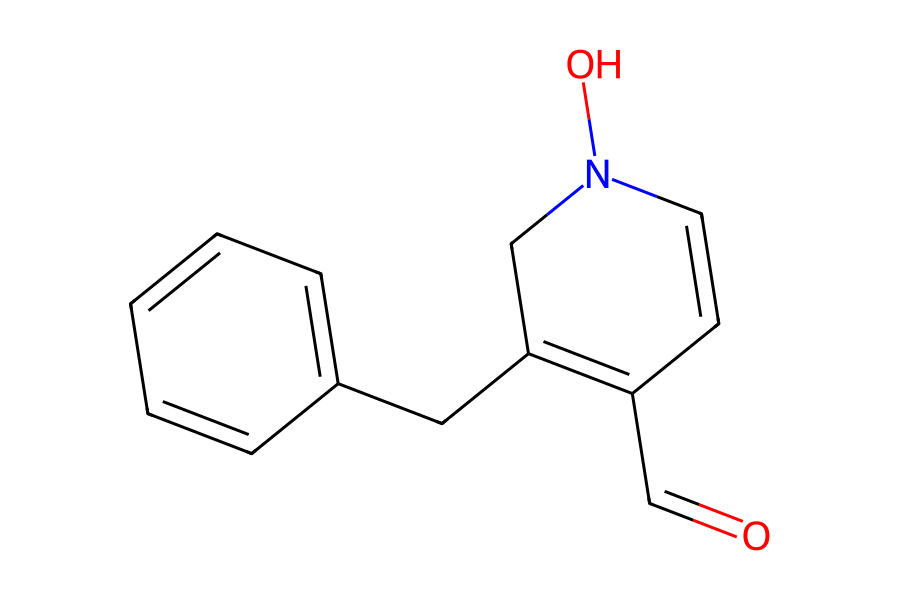
\includegraphics[width=\linewidth]{fig_ligando_2d.png}
\captionof{figure}{Estructura 2D de Macaridine.}
\label{fig:lig2d}
\end{minipage}\hfill
\begin{minipage}[c]{0.54\textwidth}
\centering
\small
\begin{tabular}{@{}ll@{}}
\toprule
Propiedad & Valor \\
\midrule
Fórmula & C$_{13}$H$_{13}$NO$_2$ \\
Masa molar & \SI{215.25}{g/mol} \\
Átomos pesados & 16 \\
$\log P$ (Crippen) & 1.94 \\
Donadores / aceptores de H & 1 / 3 \\
Enlaces rotables & 3 \\
TPSA & \SI{40.5}{\angstrom^2} \\
Carga neta & 0 \\
SMILES & \texttt{\scriptsize O=CC1=C(Cc2ccccc2)CN(O)C=C1} \\
\bottomrule
\end{tabular}
\captionof{table}{Propiedades del ligando (RDKit).}
\label{tab:lig}
\end{minipage}

\vspace{0.6em}
\textbf{Observación sobre el archivo de entrada.} Las coordenadas de \texttt{Data/ligand.pdb} (generadas por
SwissParam y centradas en el origen) \emph{no corresponden a una pose acoplada}: el ligando quedaba
dentro de la proteína, con 71 pares de átomos a menos de \SI{2.2}{\angstrom} del esqueleto de Lys578, Gly615 y
Ser616, a $\sim$\SI{17}{\angstrom} del sitio de ATP. La simulación anterior en Colab
(\texttt{SimulacionesRespados/94717379\_*.ipynb}) partió de esa pose. Por eso aquí se repitió el
\textit{docking}, como hace el artículo.

\textbf{Parametrización.} GAFF con cargas AM1-BCC (\texttt{antechamber}, AmberTools 26); parámetros
faltantes con \texttt{parmchk2} (solo un ángulo c3--nh--oh y siete impropios genéricos, todos de baja
penalización). El artículo usa GAFF con Antechamber de AMBER 20.

\subsection{\textit{Docking} con AutoDock Vina}

\begin{table}[H]
\centering\small
\begin{tabularx}{\textwidth}{@{}lXX@{}}
\toprule
Parámetro & Artículo & Esta ejecución \\
\midrule
Programa & AutoDock Vina & AutoDock Vina 1.2.7 \\
Receptor & BRAF V600E, PDB 4XV2 (cristal) & BRAF V600E, modelo SWISS-MODEL (448--723) \\
Centro de la caja & átomo F39 de dabrafenib & centroide de Ile463, Val471, Ala481, Lys483, Leu505, Leu514, Thr529, Trp531, Cys532, Phe583, Asp594 \\
Tamaño de la caja & $20\times20\times20$\,\AA$^3$ & $20\times20\times20$\,\AA$^3$ \\
\textit{Exhaustiveness} / modos & 100 / 100 & 100 / 100 (91 poses en la ventana de energía) \\
Preparación & AutoDock Tools (Gasteiger) & Open Babel (Gasteiger), semilla 42 \\
\bottomrule
\end{tabularx}
\caption{Parámetros de \textit{docking}.}
\label{tab:dock}
\end{table}

\subsection{Construcción del sistema solvatado}

\begin{table}[H]
\centering\small
\begin{tabular}{@{}lll@{}}
\toprule
Componente & Valor & Detalle \\
\midrule
Proteína & 276 residuos, 4\,459 átomos & dominio quinasa 448--723, ff19SB \\
Ligando & 29 átomos (16 pesados) & residuo \texttt{LIG}, GAFF/AM1-BCC \\
Agua & 14\,823 moléculas TIP3P & 14\,903 iniciales; 80 sustituidas por iones \\
Iones & 36 Na$^+$ + 44 Cl$^-$ & neutraliza la carga $+8$ y da NaCl 0.15 M \\
Caja & octaedro truncado & $a=\SI{89.47}{\angstrom}$, $\alpha=\beta=\gamma=\ang{109.47}$, \SI{12}{\angstrom} al borde \\
Total & \textbf{49\,037 átomos} & carga final 0 \\
Volumen inicial / final & \SI{551.3}{nm^3} / \SI{495.7}{nm^3} & densidad 0.907 $\rightarrow$ \SI{1.009}{g/mL} \\
\bottomrule
\end{tabular}
\caption{Composición del sistema (\texttt{tleap}, AmberTools 26).}
\label{tab:sistema}
\end{table}

\textbf{Número de iones (SLTCAP, Machado y Pantano).} Con $N_w$ moléculas de agua, concentración
$c$ y carga del soluto $Q$:
\begin{equation}
N_0 = \frac{N_w\,c}{\SI{55.5}{M}},\qquad y=\frac{Q}{2N_0},\qquad
N_{\pm}=N_0\left(\sqrt{1+y^2}\mp y\right).
\end{equation}
Con $N_w=14\,903$, $c=\SI{0.15}{M}$ y $Q=+8$: $N_0=40.3$, $N_+=36$ (Na$^+$), $N_-=44$ (Cl$^-$). El
artículo neutralizó una carga de $+6$ con seis Cl$^-$ (su construcción de 4XV2 tiene otra extensión).

\subsection{Protocolo de dinámica molecular}

\begin{table}[H]
\centering\small
\begin{tabularx}{\textwidth}{@{}l>{\raggedright\arraybackslash}X>{\raggedright\arraybackslash}X@{}}
\toprule
Parámetro & Artículo (sección 2.1.3) & Esta ejecución (prueba rápida) \\
\midrule
Motor & Amber (pmemd) & OpenMM 8.6.1 (plataforma CPU, 2 hilos) sobre topología AMBER \\
Minimización & 10\,000 ciclos (4000 SD + 6000 CG), restricción $k=\SI{10}{kcal\,mol^{-1}\,\angstrom^{-2}}$ en proteína y ligando & 10\,000 iteraciones L-BFGS, misma restricción ($k\,\Delta r^2$) sobre átomos pesados de proteína y ligando \\
Calentamiento & 0 $\rightarrow$ \SI{310}{K} escalonado en \SI{500}{ps}, sin restricciones & 0 $\rightarrow$ \SI{310}{K} en 31 escalones de \SI{10}{K}, \textbf{\SI{20}{ps}}, NVT, sin restricciones \\
Equilibrado & \SI{500}{ps} & \textbf{\SI{20}{ps}}, NPT \SI{310}{K}, \SI{1}{atm} \\
Producción & \SI{1}{\micro s} NPT (\SI{300}{ns} dabrafenib) & \textbf{\SI{100}{ps}} NPT, 4 segmentos de \SI{25}{ps} \\
Temperatura & \SI{310}{K} & \SI{310}{K} \\
Termostato & Langevin, $\gamma=\SI{1}{ps^{-1}}$ & Langevin (\texttt{LangevinMiddle}), $\gamma=\SI{1}{ps^{-1}}$ \\
Presión & \SI{1}{atm} & \SI{1}{atm}, barostato Monte Carlo (cada 25 pasos) \\
Paso de integración & \SI{2}{fs} & \SI{2}{fs} \\
Restricciones & SHAKE en enlaces con H & enlaces con H rígidos (tolerancia $10^{-6}$), agua rígida \\
Corte no enlazado & \SI{11}{\angstrom} & \SI{11}{\angstrom} \\
Largo alcance & PME & PME (tolerancia de Ewald $5\times10^{-4}$) \\
Contorno & periódico en x, y, z & periódico, octaedro truncado \\
Guardado & no indicado & 1 fotograma/ps (proteína + ligando en producción) \\
\bottomrule
\end{tabularx}
\caption{Parámetros de simulación: artículo frente a esta ejecución. Por ser una prueba rápida, solo
se acortaron las duraciones de calentamiento, equilibrado y producción.}
\label{tab:md}
\end{table}

\subsection{Software y equipo}

AmberTools 26 (\texttt{tleap}, \texttt{antechamber}, \texttt{parmchk2}, \texttt{MMPBSA.py}),
OpenMM 8.6.1, PDB2PQR 3.6.1 + PROPKA, AutoDock Vina 1.2.7, Open Babel, RDKit 2026.03, ParmEd 4.3.1,
MDAnalysis 2.10, MDTraj y PyMOL (versión libre). Equipo: 2 núcleos virtuales Intel Xeon a \SI{2.1}{GHz}
sin GPU. Velocidad: 1.10~ns/día en NVT y 0.81--0.88~ns/día en NPT. Duración real:
minimización 13~min, calentamiento + equilibrado 1~h, producción 3.2~h.

\subsection{Incidencia durante la ejecución}

El segundo segmento de producción se detuvo a los $\sim$\SI{28}{ps} por coordenadas no numéricas (NaN).
El estado guardado justo antes estaba limpio: ningún par de átomos no enlazados a menos de
\SI{1.3}{\angstrom}, geometría del ligando normal, y temperatura y densidad estables. El segmento se repitió
desde el último punto de control y completó los \SI{100}{ps} sin más problemas. El script ahora
reintenta automáticamente un segmento con NaN y lo anota en \texttt{md\_prueba/incidencias.log}.

% =====================================================================
\section{Resultados}
% =====================================================================

\subsection{Pose de partida (\textit{docking})}

La mejor pose obtuvo \textbf{\SI{-7.38}{kcal/mol}}; las 91 poses quedaron entre $-7.38$ y
\SI{-5.64}{kcal/mol} (figura~\ref{fig:vina}). La mejor pose sitúa el ligando en el bolsillo de ATP, entre
el lóbulo N (lámina $\beta$, lazo rico en glicinas y Lys483) y el lóbulo C, junto a la bisagra
(figura~\ref{fig:complejo}).

Como referencia, en el artículo el dabrafenib obtuvo \SI{-12.7}{kcal/mol} y sus cuatro mejores
compuestos menos de \SI{-12}{kcal/mol}, aunque con otro receptor (estructura cristalina). Macaridine es
una molécula pequeña (16 átomos pesados frente a 35 del dabrafenib): por átomo pesado su puntuación es
$-0.46$ frente a \SI{-0.36}{kcal/mol}, pero su afinidad total predicha es mucho menor.

\begin{figure}[H]
\centering
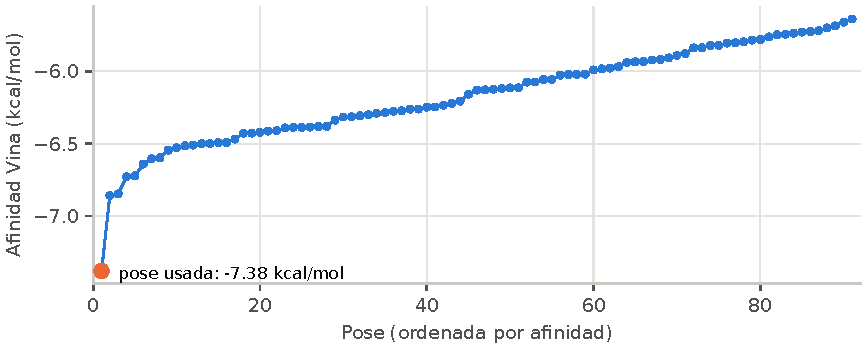
\includegraphics[width=0.92\textwidth]{fig_vina.pdf}
\caption{Afinidad de las 91 poses de Vina, ordenadas. El punto naranja marca la pose usada para la MD.}
\label{fig:vina}
\end{figure}

\begin{figure}[H]
\centering
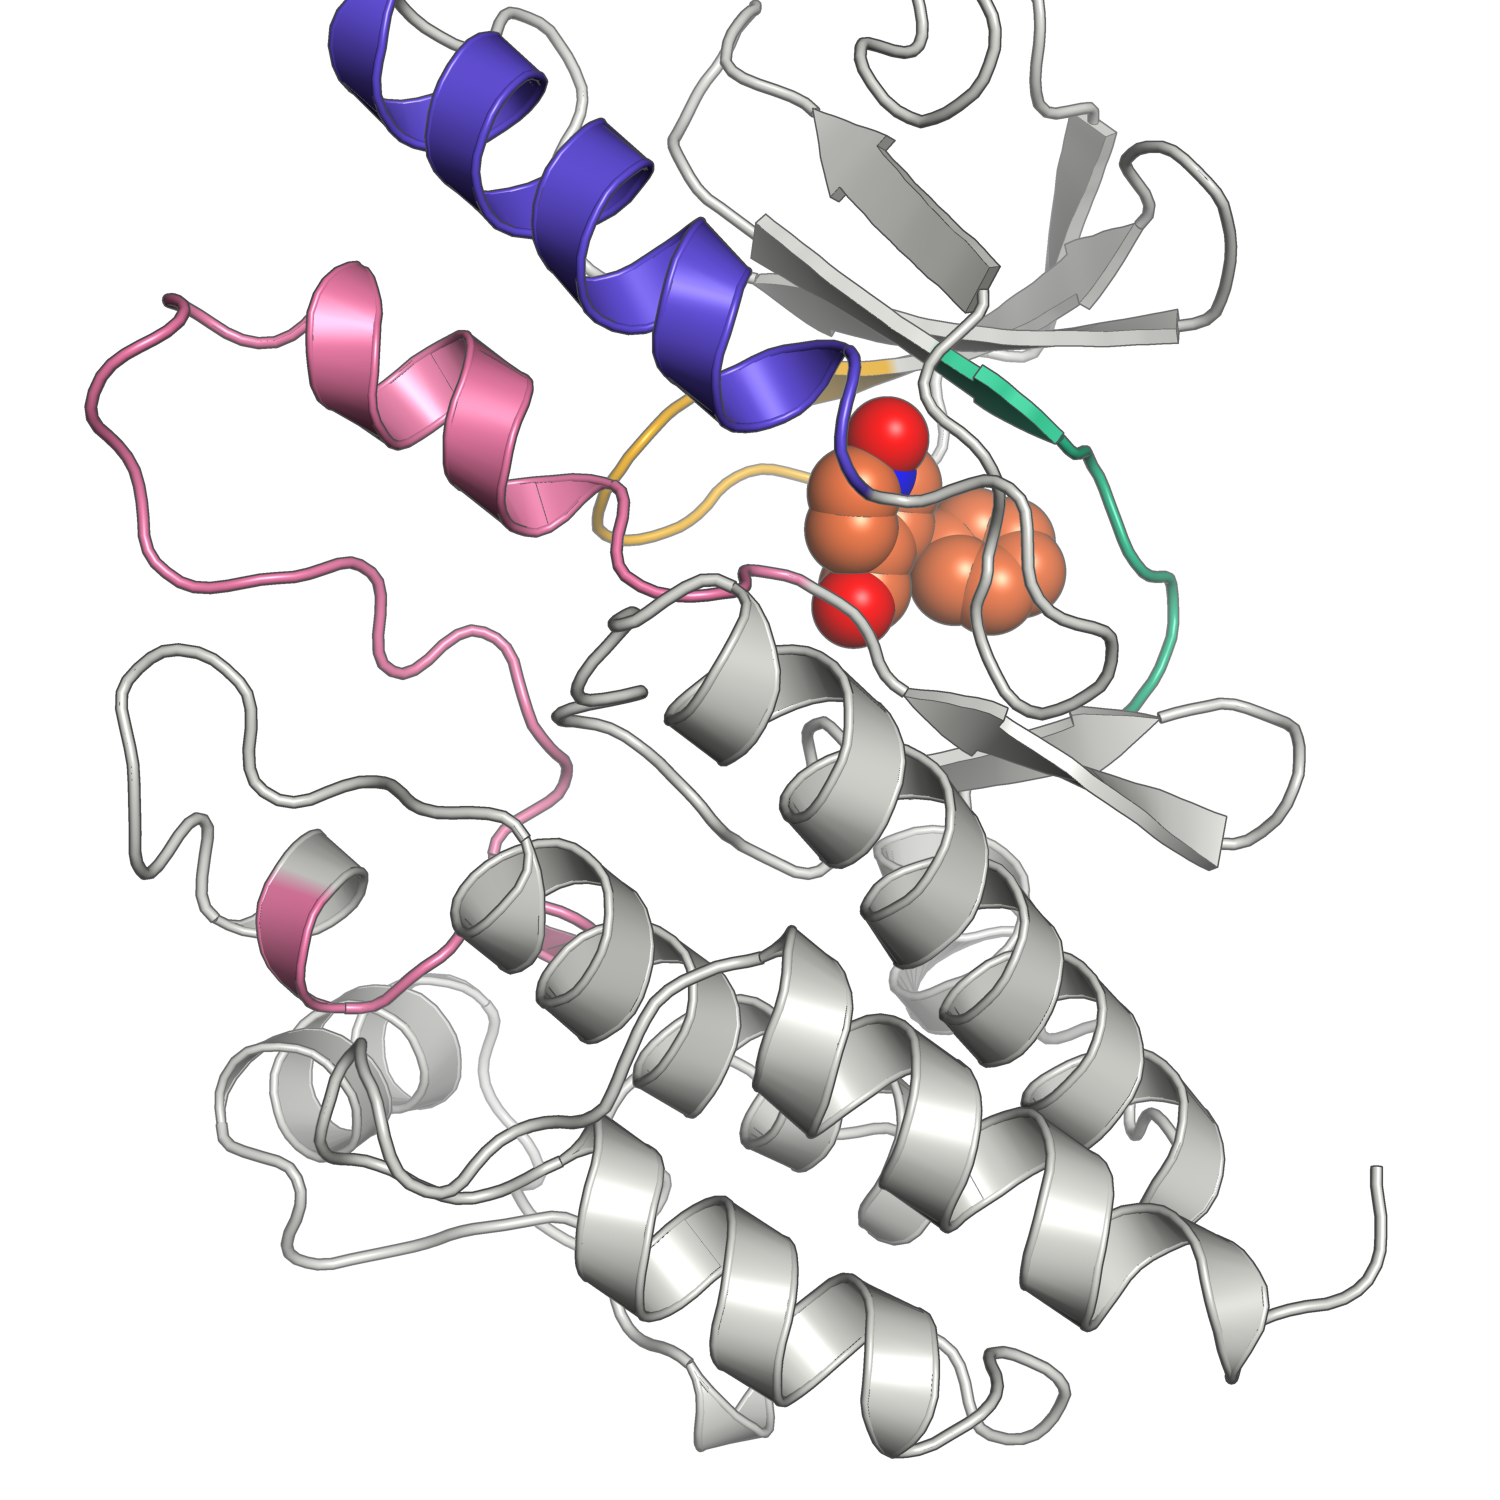
\includegraphics[width=0.62\textwidth]{fig_complejo_general.png}
\caption{Complejo al final de la producción. Dominio quinasa de BRAF V600E en gris; lazo rico en
glicinas (464--471) en amarillo; hélice $\alpha$C (492--507) en violeta; bisagra (529--535) en verde;
DFG y lazo de activación (594--623) en rosa; Macaridine en esferas naranjas, en la hendidura entre los
lóbulos.}
\label{fig:complejo}
\end{figure}

\subsection{Minimización y estabilidad termodinámica}

La minimización bajó la energía potencial de \SI{-549934}{kJ/mol} a \SI{-800107}{kJ/mol}, eliminando
los choques que dejaron los hidrógenos añadidos por \texttt{tleap}. La figura~\ref{fig:termo} muestra
las variables de control en las tres etapas:

\begin{itemize}
\item \textbf{Temperatura:} sube de forma lineal hasta \SI{310}{K} en el calentamiento y se mantiene en
      \SI{310.5 \pm 1.5}{K} en producción.
\item \textbf{Densidad y volumen:} constantes en el calentamiento (NVT). Al activar el barostato, la caja
      se contrae un 10\,\% y la densidad pasa de 0.907 a \SI{1.009 \pm 0.002}{g/mL} en unos \SI{15}{ps};
      después queda estable. La densidad inicial baja es normal en cajas recién construidas con
      \texttt{tleap}.
\item \textbf{Energía potencial:} sube con la temperatura y se estabiliza en
      \SI{-653400 \pm 900}{kJ/mol}, sin derivas.
\end{itemize}

\begin{figure}[H]
\centering
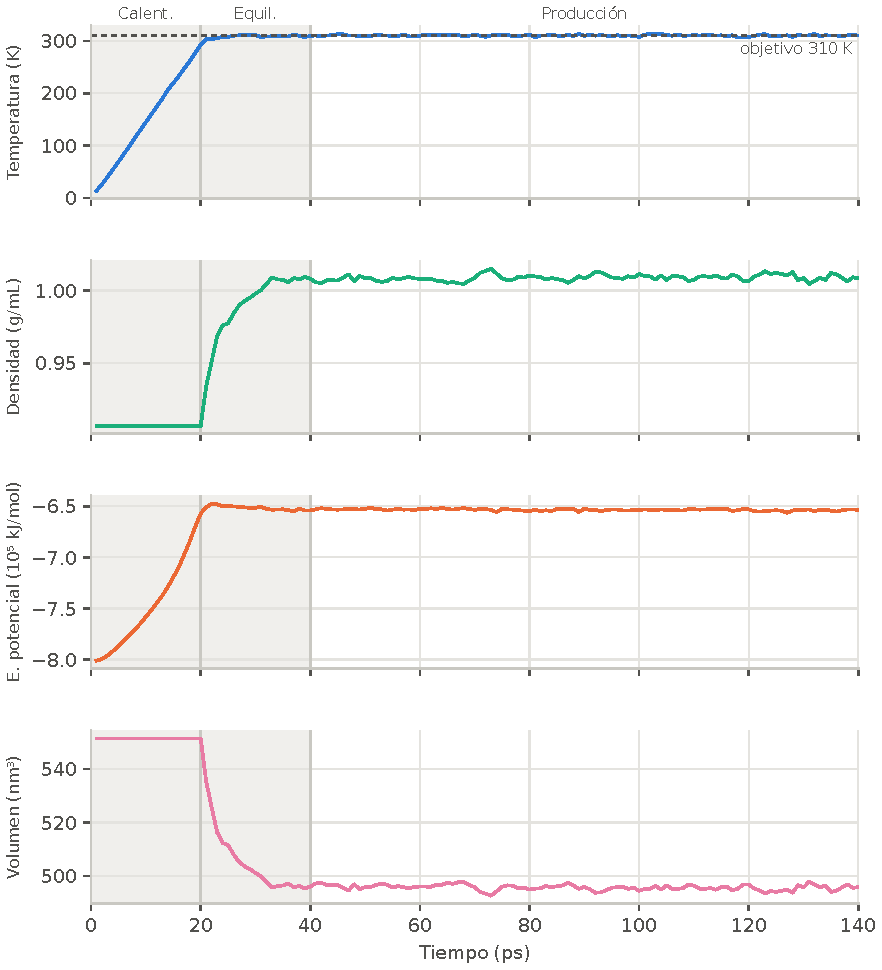
\includegraphics[width=0.9\textwidth]{fig_termodinamica.pdf}
\caption{Temperatura, densidad, energía potencial y volumen de la caja. Fondo gris: calentamiento (NVT,
0--20 ps) y equilibrado (NPT, 20--40 ps); fondo blanco: producción (NPT, 40--140 ps).}
\label{fig:termo}
\end{figure}

\subsection{RMSD de la proteína y del ligando}

\begin{figure}[H]
\centering
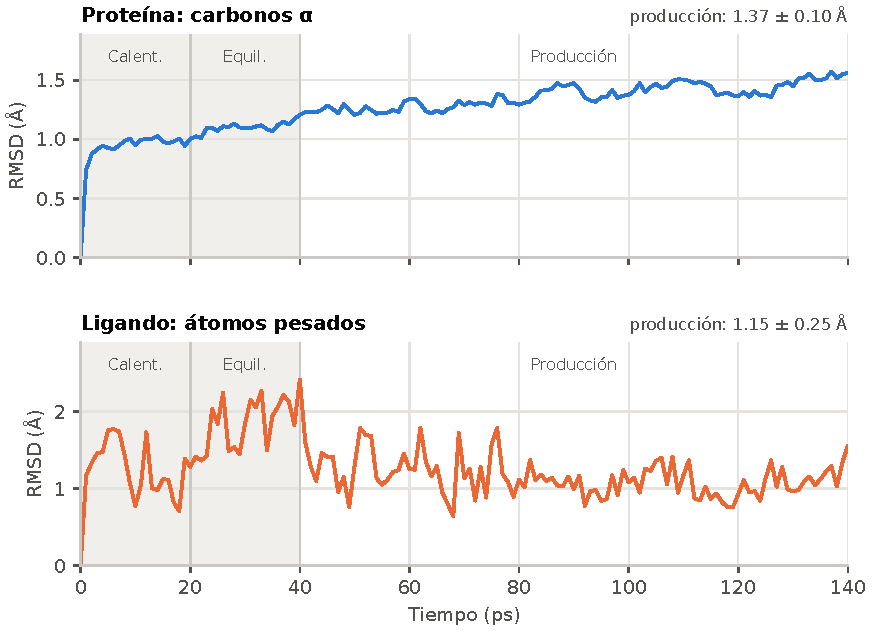
\includegraphics[width=0.92\textwidth]{fig_rmsd.pdf}
\caption{RMSD respecto a la estructura minimizada. Arriba: carbonos $\alpha$ de la proteína. Abajo:
átomos pesados del ligando tras superponer la proteína (desplazamiento dentro del bolsillo).}
\label{fig:rmsd}
\end{figure}

\begin{table}[H]
\centering\small
\begin{tabular}{@{}lccc@{}}
\toprule
RMSD (\AA) & Calentamiento & Equilibrado & Producción \\
\midrule
Proteína, \Ca & $0.96 \pm 0.06$ & $1.10 \pm 0.04$ & $\mathbf{1.37 \pm 0.10}$ (máx.\ 1.57) \\
Ligando, átomos pesados & $1.26 \pm 0.33$ & $1.86 \pm 0.34$ & $\mathbf{1.15 \pm 0.25}$ (máx.\ 1.79) \\
\bottomrule
\end{tabular}
\caption{RMSD medio $\pm$ desviación estándar por etapa.}
\label{tab:rmsd}
\end{table}

\begin{itemize}
\item \textbf{Proteína:} el RMSD sube rápido a $\sim$\SI{1}{\angstrom} al liberar las restricciones y luego
      crece lentamente, hasta \SI{1.56}{\angstrom} al final, a un ritmo de $\sim$\SI{0.3}{\angstrom} cada
      \SI{100}{ps}. \emph{No llega a una meseta}, lo esperable en \SI{100}{ps}. En el artículo, el
      complejo con su mejor compuesto (T160) osciló alrededor de \SI{2.44}{\angstrom} durante \SI{900}{ns}. Los
      valores de \SIrange{1}{2}{\angstrom} son típicos de un dominio quinasa bien plegado.
\item \textbf{Ligando:} se mueve más en el equilibrado (hasta \SI{2.4}{\angstrom}, mientras la caja se
      contrae) y se reacomoda en producción, donde se mantiene en \SI{1.15 \pm 0.25}{\angstrom}. \emph{No hay
      tendencia a salir del bolsillo}: un ligando que se disocia muestra saltos de varios Å.
\end{itemize}

\subsection{Compacidad y estructura secundaria}

El radio de giro de la proteína fue \SI{19.34 \pm 0.06}{\angstrom} en producción (figura~\ref{fig:rg}),
prácticamente el del artículo para T160 (de 19.24 a \SI{19.15}{\angstrom}). La proteína no se expande ni se
compacta. Según DSSP, la estructura secundaria se conservó: hélices 38.8\,\% $\rightarrow$ 38.0\,\%,
láminas $\beta$ 15.6\,\% $\rightarrow$ 13.4\,\% y lazos 45.7\,\% $\rightarrow$ 48.6\,\% entre el
primer y el último fotograma de producción.

\begin{figure}[H]
\centering
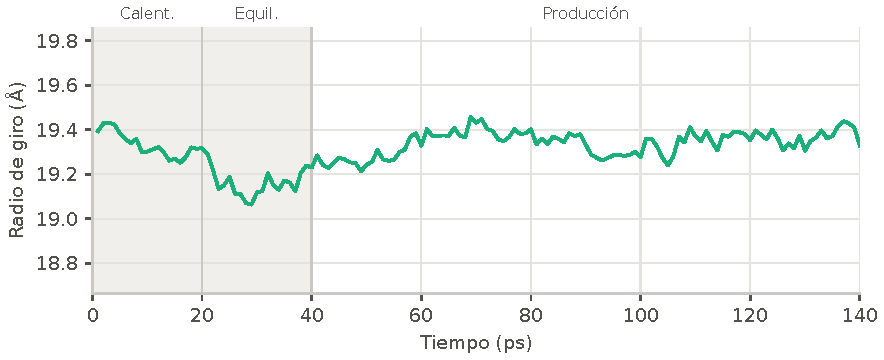
\includegraphics[width=0.92\textwidth]{fig_rg.pdf}
\caption{Radio de giro de la proteína (todos los átomos).}
\label{fig:rg}
\end{figure}

\subsection{Flexibilidad por residuo (RMSF)}

\begin{figure}[H]
\centering
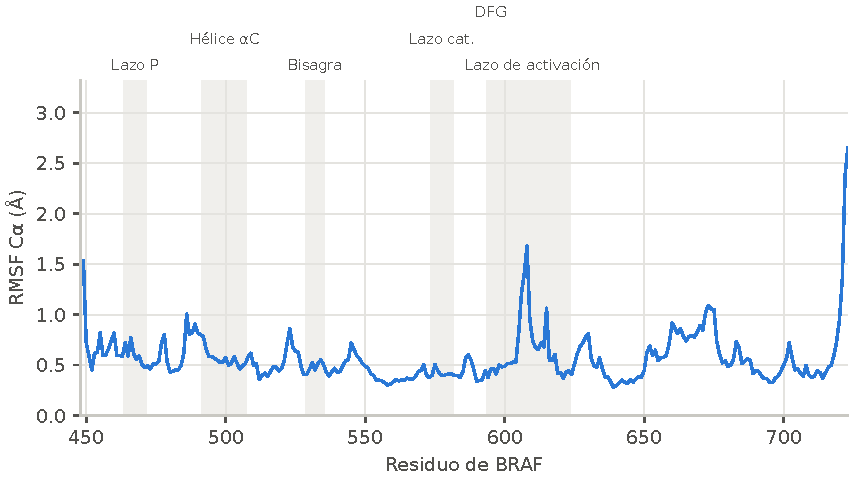
\includegraphics[width=0.95\textwidth]{fig_rmsf.pdf}
\caption{RMSF de los \Ca{} en producción, con las regiones funcionales del dominio quinasa sombreadas
(numeración aproximada).}
\label{fig:rmsf}
\end{figure}

El RMSF medio fue \SI{0.57}{\angstrom}. Lo más móvil son los extremos recortados (Asp448--449 y
Leu721--Lys723, \SIrange{1.4}{2.7}{\angstrom}), lo esperable en extremos libres, y un segmento del
\textbf{lazo de activación}, Gly606--His608 (pico de \SI{1.7}{\angstrom}). El artículo identificó justo ese
segmento (Ser607--Ser614) como uno de los más flexibles (> \SI{3}{\angstrom} en \SI{1}{\micro s}). Las regiones
que tocan al ligando son rígidas: bisagra \SI{0.49}{\angstrom}, DFG \SI{0.44}{\angstrom}, lazo catalítico
\SI{0.42}{\angstrom}, lazo rico en glicinas \SI{0.60}{\angstrom} y hélice $\alpha$C \SI{0.56}{\angstrom}. El artículo
también reporta RMSF $<\SI{1}{\angstrom}$ para Asp594--Gly596.

\subsection{Interacciones ligando--proteína}

\begin{figure}[H]
\centering
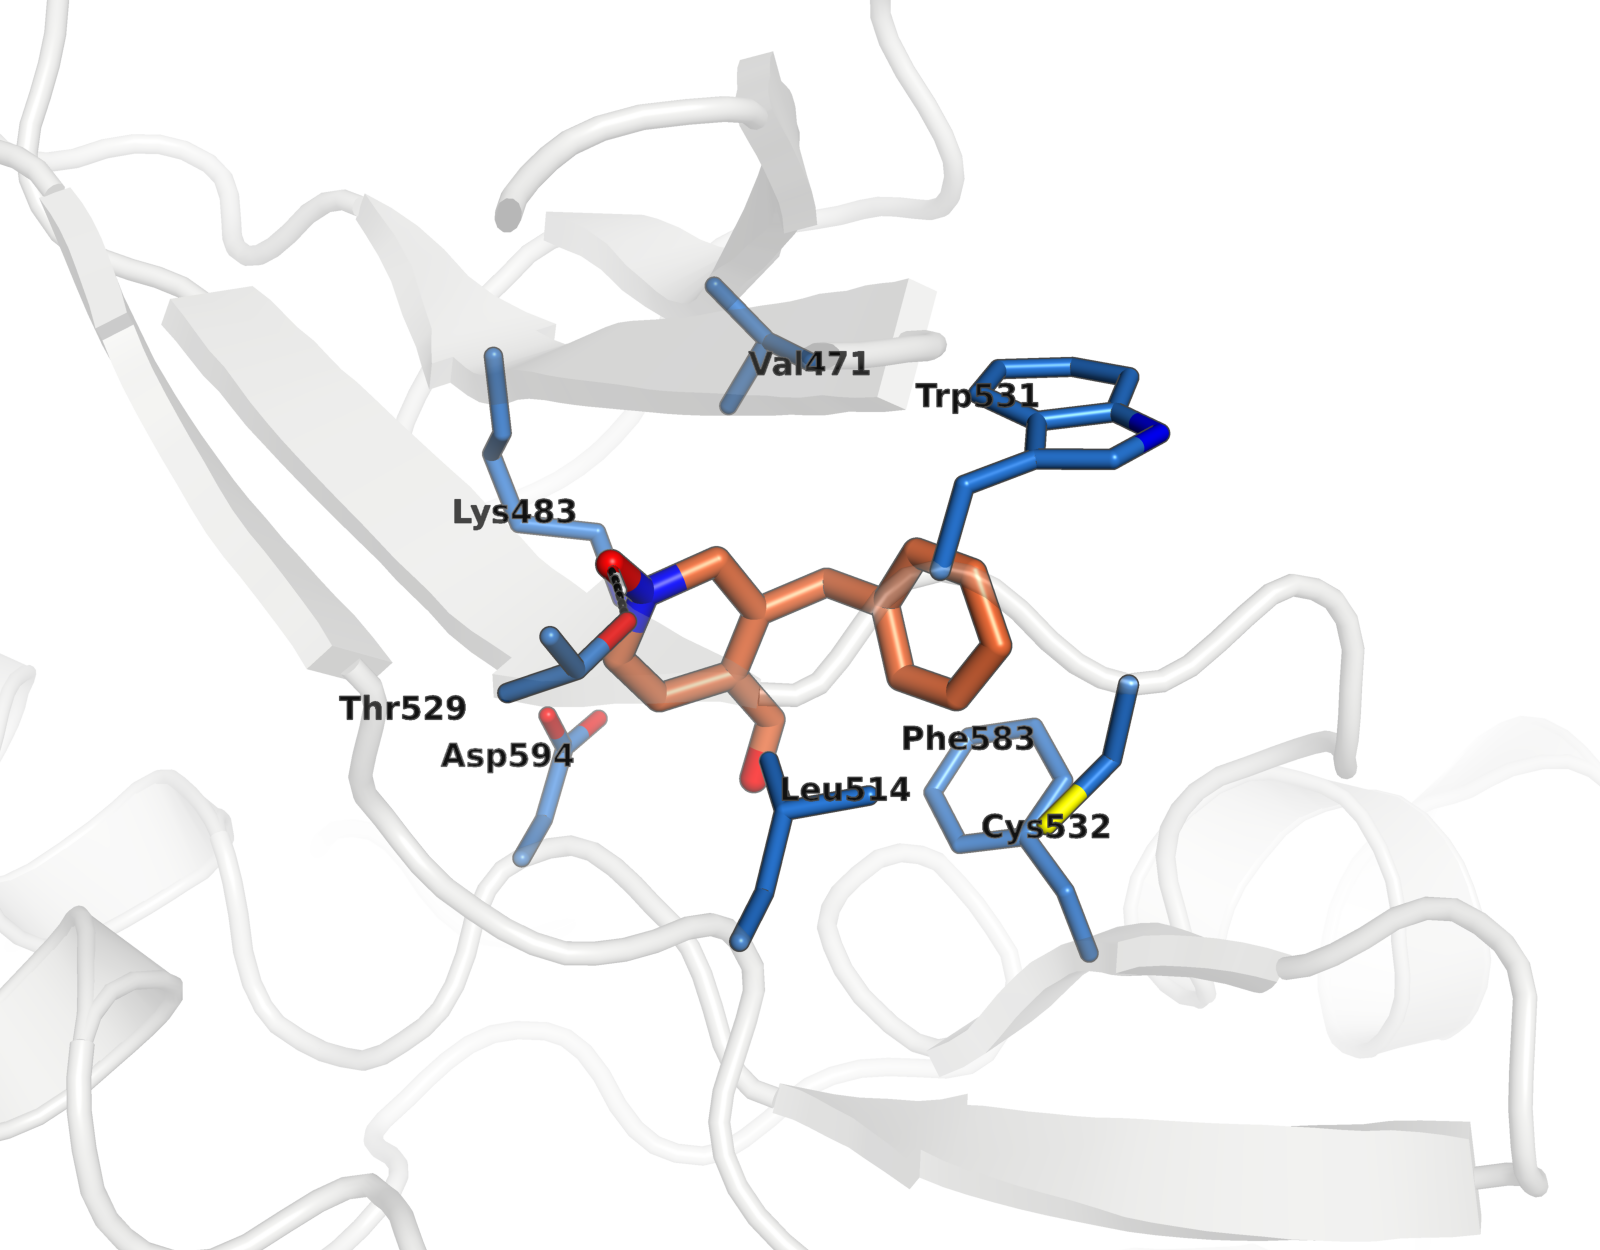
\includegraphics[width=0.78\textwidth]{fig_bolsillo.png}
\caption{Bolsillo de unión al final de la simulación. Macaridine en naranja; residuos en contacto en
azul. Línea discontinua: puente de hidrógeno entre el grupo N--OH del ligando y el hidroxilo de Thr529
(\emph{gatekeeper}).}
\label{fig:bolsillo}
\end{figure}

\begin{figure}[H]
\centering
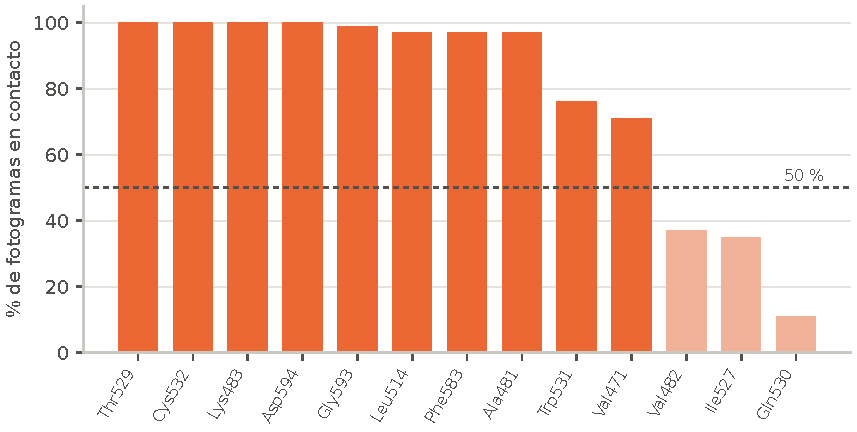
\includegraphics[width=0.92\textwidth]{fig_contactos.pdf}
\caption{Porcentaje de fotogramas de producción en que cada residuo está a menos de \SI{4}{\angstrom} del
ligando. En naranja intenso, los contactos presentes en más del 50\,\% del tiempo.}
\label{fig:contactos}
\end{figure}

\begin{itemize}
\item \textbf{Puente de hidrógeno:} el hidroxilo del grupo N--OH de Macaridine dona un puente de
      hidrógeno al oxígeno O$\gamma$1 de \textbf{Thr529} en el \textbf{99\,\%} de los fotogramas. Thr529
      es el residuo \emph{gatekeeper}, que controla el acceso al bolsillo hidrofóbico posterior. El
      artículo describe un puente de hidrógeno con Thr529 como la interacción predominante de su mejor
      compuesto, T160 (75\,\% del tiempo).
\item \textbf{Contactos permanentes} ($\ge$97\,\% del tiempo): Lys483 (lisina catalítica de la hebra
      $\beta$3), Thr529, Cys532 (bisagra), Gly593 y Asp594 (motivo DFG), Leu514, Phe583 y Ala481.
      Frecuentes: Trp531 (76\,\%) y Val471 (71\,\%).
\item \textbf{Comparación con el artículo:} para T160, los residuos con mayor contribución a la unión
      fueron Thr529, Lys483, Val471, Leu505, Leu514, Trp531 y Phe583; para dabrafenib, Gly593, Phe583,
      Trp531, Val471, Leu514, Ile527, Thr529 y Cys532. Macaridine ocupa el mismo sitio y toca casi los
      mismos residuos.
\item \textbf{Enterramiento:} el \SI{94.6 \pm 1.2}{\percent} de la superficie del ligando
      (\SI{431}{\angstrom^2} libre) queda cubierto por la proteína.
\end{itemize}

\begin{figure}[H]
\centering
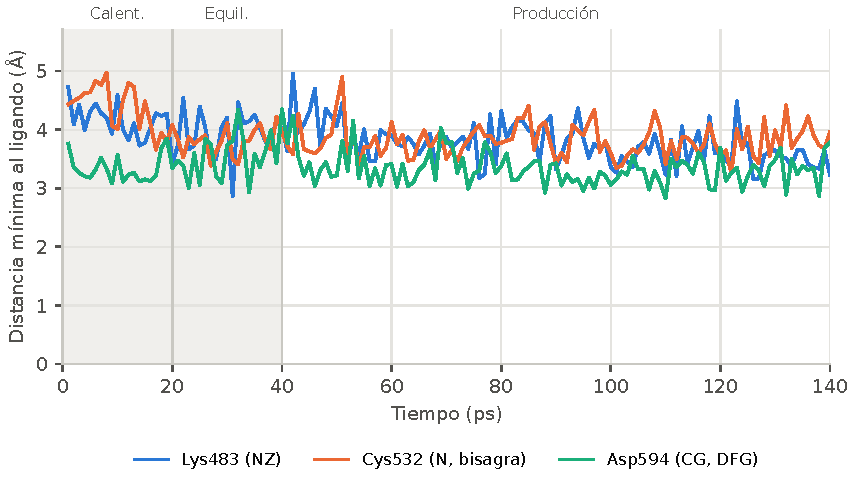
\includegraphics[width=0.92\textwidth]{fig_distancias.pdf}
\caption{Distancia mínima entre el ligando y tres anclajes del bolsillo: Lys483, Cys532 (bisagra) y
Asp594 (DFG).}
\label{fig:dist}
\end{figure}

Las distancias a los tres anclajes se mantienen entre 3 y \SI{5}{\angstrom} durante toda la simulación
(producción: Lys483 \SI{3.75 \pm 0.35}{\angstrom}, Cys532 \SI{3.81 \pm 0.28}{\angstrom}, Asp594
\SI{3.33 \pm 0.27}{\angstrom}). Ninguna crece de forma sostenida, lo que confirma que el ligando permanece
anclado en el sitio de ATP.

\subsection{Energía libre de unión (MM/GBSA)}
\label{sec:mmgbsa}

Sobre los 100 fotogramas de producción se aplicó MM/GBSA (\texttt{MMPBSA.py}, modelo GB-OBC2
\texttt{igb=5}, radios mbondi2, sal \SI{0.15}{M}, sin entropía, como en el artículo).

\begin{table}[H]
\centering\small
\begin{tabular}{@{}lr@{}}
\toprule
Término & $\Delta$ (kcal\,mol$^{-1}$) \\
\midrule
van der Waals ($\Delta E_{\text{vdW}}$) & \GBvdw \\
Electrostática ($\Delta E_{\text{elec}}$) & \GBeel \\
Solvatación polar ($\Delta G_{\text{GB}}$) & \GBegb \\
Solvatación no polar ($\Delta G_{\text{SA}}$) & \GBesurf \\
\midrule
Fase gas ($\Delta E_{\text{MM}}$) & \GBgas \\
Solvatación total ($\Delta G_{\text{solv}}$) & \GBsolv \\
\midrule
$\boldsymbol{\Delta G_{\text{unión}}}$ (sin $-T\Delta S$) & $\mathbf{\GBtotal \pm \GBsd}$ (e.e.m.\ \GBsem) \\
\bottomrule
\end{tabular}
\caption{MM/GBSA de Macaridine--BRAF V600E (media $\pm$ desviación estándar entre fotogramas).}
\label{tab:mmgbsa}
\end{table}

El balance es favorable: $\Delta G_{\text{unión}} = \SI{-27.4 \pm 2.9}{kcal/mol}$. Lo que más
aporta son las fuerzas de van der Waals ($\SI{-30.9}{kcal/mol}$), es decir, el buen encaje del ligando
en el bolsillo hidrofóbico. La atracción electrostática ($\SI{-15.0}{kcal/mol}$) se compensa en gran
parte con el costo de quitar el agua a los grupos polares ($\SI{+23.2}{kcal/mol}$).

La descomposición por residuo (figura~\ref{fig:mmgbsa}) señala como \emph{dominantes} (umbral de
\SI{-1.5}{kcal/mol}, como en el artículo) a \textbf{Thr529} ($-3.1$, casi todo electrostático: es el
puente de hidrógeno), \textbf{Lys483} ($-2.7$) y \textbf{Leu514} ($-1.9$). Gly593 queda justo en el
límite ($-1.50$) y les siguen Phe583, Val471 y Ala481 (entre $-1.2$ y $-1.4$). Son prácticamente los
mismos residuos dominantes que el artículo reporta para su compuesto T160: Thr529, Lys483, Val471,
Leu505, Leu514, Trp531 y Phe583.

\textbf{Escala de referencia.} El artículo obtuvo \SI{-59.1 \pm 2.6}{kcal/mol} para T160,
\SI{-61.7 \pm 1.0}{kcal/mol} para dabrafenib y \SI{-39.7 \pm 2.2}{kcal/mol} para T126, con trayectorias
de \SI{300}{ns} a \SI{1}{\micro s}. Macaridine queda en menos de la mitad, algo coherente con su
tamaño. Dividido entre átomos pesados da \SI{-1.71}{kcal/mol} por átomo, frente a \SI{-1.76}{kcal/mol}
del dabrafenib (35 átomos pesados): Macaridine aprovecha bien su tamaño, pero su afinidad total
estimada es mucho menor. Además, estos números salen de \SI{100}{ps} y de un receptor modelado, así que
son solo orientativos.

\begin{figure}[H]
\centering
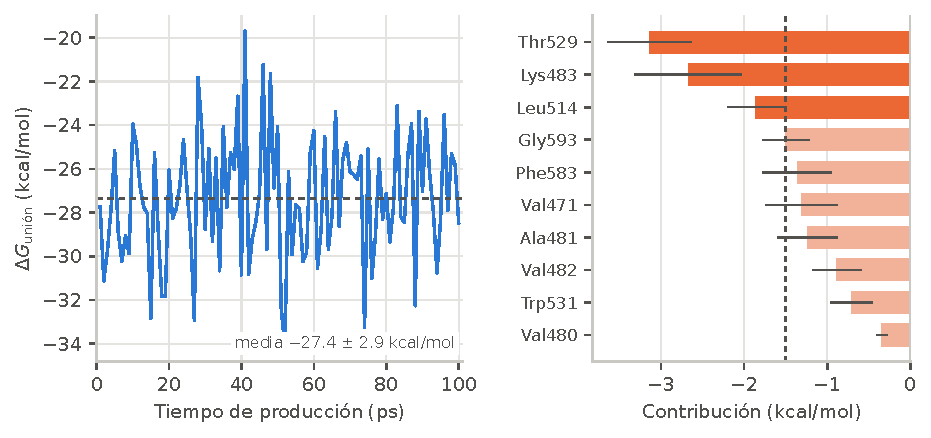
\includegraphics[width=0.95\textwidth]{fig_mmgbsa.pdf}
\caption{Izquierda: $\Delta G_{\text{unión}}$ por fotograma de producción. Derecha: residuos con mayor
contribución según la descomposición por residuo; la línea discontinua marca el umbral de
\SI{-1.5}{kcal/mol} que usa el artículo para residuos \emph{dominantes}.}
\label{fig:mmgbsa}
\end{figure}

% =====================================================================
\section{Discusión y limitaciones}
% =====================================================================

\begin{enumerate}
\item \textbf{Duración.} \SI{100}{ps} de producción son unas $10^4$ veces menos que el \SI{1}{\micro s}
      del artículo. Basta para validar el protocolo y ver que el complejo no se desarma de inmediato,
      pero no para observar cambios lentos (movimientos del lazo de activación o de la hélice $\alpha$C,
      salida del ligando) ni para que el RMSD llegue a una meseta. Los valores de MM/GBSA con 100
      fotogramas tan cercanos en el tiempo están correlacionados y no son una estimación convergida.
\item \textbf{Una sola réplica} y una sola pose de partida; no se estima la variabilidad entre
      trayectorias.
\item \textbf{Modelo del receptor.} Es un modelo por homología, no la estructura cristalina 4XV2 del
      artículo, y está recortado (448--723). Las puntuaciones de \textit{docking} y las energías no son
      directamente comparables con las del artículo.
\item \textbf{Protonación de Glu600.} PROPKA asignó Glu600 neutro (GLH) en este modelo. Conviene revisarlo: lo
      habitual es simular Glu600 cargado, y su estado puede influir en la dinámica del lazo de activación
      (aunque no está en contacto directo con el ligando).
\item \textbf{Diferencias técnicas con el artículo:} minimizador L-BFGS en lugar de SD + CG, OpenMM en
      lugar de pmemd y barostato de Monte Carlo. Son equivalentes en propósito y no deberían cambiar las
      conclusiones.
\item \textbf{Incidencia NaN:} un evento aislado en el segmento 2, resuelto al repetirlo. Si se repite
      en la corrida larga, hay que investigarlo (p.\ ej.\ con precisión doble o un paso de \SI{1}{fs}).
\end{enumerate}

% =====================================================================
\section{Conclusión para biología}
% =====================================================================

\begin{center}
\fcolorbox{aqua!60!black}{aqua!6}{\begin{minipage}{0.94\textwidth}
\textbf{¿Qué se hizo?} Se tomó un modelo 3D de BRAF con la mutación V600E (la de muchos melanomas), se
colocó la molécula Macaridine en el lugar donde normalmente se une el ATP (el ``combustible'' que la
quinasa usa para activar a sus proteínas blanco) y se simuló en computadora, átomo por átomo, cómo se
mueve ese complejo en agua salina a temperatura corporal (\SI{37}{\celsius}).

\textbf{¿Qué se vio?}
\begin{itemize}[leftmargin=1.2em]
\item La proteína se mantuvo bien plegada y estable durante toda la simulación.
\item Macaridine \textbf{se quedó dentro del bolsillo del ATP}, sin intentar salir, y quedó cubierta
      en un 95\,\% por la proteína.
\item Se sujeta mediante un \textbf{puente de hidrógeno muy estable con Thr529}, el residuo
      ``portero'' del bolsillo, y mediante contactos con Lys483, la bisagra (Cys532, Trp531) y el motivo
      DFG (Asp594). Son los mismos puntos de anclaje que usan los inhibidores aprobados, como el
      dabrafenib, y los compuestos diseñados en el artículo.
\item Las zonas que se mueven más (extremos de la cadena y parte del lazo de activación) están lejos
      del ligando, igual que en el artículo.
\end{itemize}

\textbf{¿Qué significa?} Es una señal \emph{compatible} con que Macaridine pueda ocupar el sitio de ATP
de BRAF V600E y, por tanto, competir con el ATP. Pero es una molécula pequeña (215 Da) y su puntuación
de \textit{docking} ($-7.4$ kcal/mol) y su energía de unión estimada ($-27$ kcal/mol por MM/GBSA)
están bastante por debajo de las de los inhibidores optimizados del artículo ($\le -12$ y $\sim -60$
kcal/mol, respectivamente). Lo más probable es que, si actúa, sea un inhibidor débil o un punto
de partida (``fragmento'') para diseñar derivados más potentes.

\textbf{¿Qué NO se puede concluir todavía?} Con \SI{0.1}{ns} de simulación no se puede afirmar que la
unión sea estable a largo plazo ni cuantificar la afinidad. Tampoco se puede decir que Macaridine
inhiba a BRAF en la célula: eso requiere experimentos.

\textbf{Siguientes pasos recomendados:} (1) correr el protocolo completo (\SI{0.5}{ns} +
\SI{0.5}{ns} + \SI{1}{\micro s}, o al menos 3 réplicas de \SIrange{100}{300}{ns}) en GPU; (2) simular
dabrafenib con el mismo protocolo como control positivo y comparar RMSD, puentes de hidrógeno y
MM/GBSA; (3) si los resultados siguen siendo favorables, validar experimentalmente con un ensayo de
actividad quinasa de BRAF V600E (IC$_{50}$) y uno de viabilidad en células de melanoma con BRAF V600E
(p.\ ej.\ A375).
\end{minipage}}
\end{center}

\clearpage
% =====================================================================
\section{Segundo compuesto: Pallidine (PubChem CID 24543347)}
\label{sec:pallidine}
% =====================================================================

\begin{center}
\fcolorbox{gris!40}{fondo}{\begin{minipage}{0.93\textwidth}
\small
\textbf{Resumen (Pallidine).} Con el mismo receptor y el mismo protocolo que Macaridine
(\SI{20}{ps} + \SI{20}{ps} + \SI{100}{ps}), Pallidine obtuvo una mejor puntuación de \textit{docking}
(\SI{-8.07}{kcal/mol}) y una energía MM/GBSA más favorable (\SI{-34.4 \pm 2.5}{kcal/mol}), sobre todo por
ser más grande. Pero su modo de unión es menos específico: el ligando se desplazó $\sim$\SI{3}{\angstrom} y
giró dentro del bolsillo de ATP (RMSD \SI{3.89 \pm 0.36}{\angstrom}, aún en aumento), perdió el contacto con
Thr529 y no formó puentes de hidrógeno estables. Se sostiene por contactos hidrofóbicos con Phe583, Leu514
y Val471. La proteína se mantuvo estable (RMSD \Ca{} \SI{1.39 \pm 0.08}{\angstrom}). Se simuló la forma
neutra; la amina protonada, probable a pH 7.4, podría anclarse a Asp594: se simuló después a \SI{50}{ns}
(sección~\ref{sec:50ns}).
\end{minipage}}
\end{center}

\subsection{Qué cambia respecto a Macaridine}

Se repitió \emph{exactamente} el mismo flujo de trabajo (figura~\ref{fig:flujo}), con los mismos scripts y
parámetros (tablas~\ref{tab:dock} y~\ref{tab:md}) y las mismas versiones de los programas principales; solo
cambia el ligando:

\begin{itemize}
\item \textbf{Receptor:} el archivo de entrada (\nolinkurl{Data/Pallidine24543347_receptor.pdb}) es idéntico,
      byte a byte, al de Macaridine. Tras el recorte (448--723) y la protonación, el archivo
      \texttt{receptor\_amber.pdb} también es idéntico al de Macaridine: mismos estados HID/HIE y
      Glu600 protonado (GLH). Las diferencias entre las dos simulaciones se deben, por tanto, solo al ligando.
\item \textbf{Ligando:} \nolinkurl{Data/Pallidine24543347_ligand.pdb} (SwissParam, 45 átomos con hidrógenos).
\item \textbf{Protocolo:} minimización de 10\,000 iteraciones, \SI{20}{ps} de calentamiento, \SI{20}{ps} de
      equilibrado y \SI{100}{ps} de producción en 4 segmentos, con los mismos parámetros físicos.
\item \textbf{Carpeta:} \nolinkurl{Simulacion/dockingML/simulaciones/Pallidine_24543347/}; figuras en
      \nolinkurl{Img/Pallidine_24543347/}.
\end{itemize}

\subsection{Ligando: Pallidine}

\begin{minipage}[c]{0.42\textwidth}
\centering
\includegraphics[width=\linewidth]{\figP{fig_ligando_2d.png}}
\captionof{figure}{Estructura 2D de Pallidine.}
\label{fig:P:lig2d}
\end{minipage}\hfill
\begin{minipage}[c]{0.54\textwidth}
\centering
\small
\begin{tabular}{@{}lll@{}}
\toprule
Propiedad & Pallidine & Macaridine \\
\midrule
Fórmula & C$_{19}$H$_{21}$NO$_4$ & C$_{13}$H$_{13}$NO$_2$ \\
Masa molar (g/mol) & 327.38 & 215.25 \\
Átomos pesados & 24 & 16 \\
$\log P$ (Crippen) & 1.94 & 1.94 \\
Donadores / aceptores de H & 1 / 5 & 1 / 3 \\
Enlaces rotables & 2 & 3 \\
TPSA (\AA$^2$) & 59.0 & 40.5 \\
Estereocentros & 2 (ambos $S$) & 0 \\
Carga neta usada & 0 & 0 \\
\bottomrule
\end{tabular}
\captionof{table}{Propiedades del ligando (RDKit).}
\label{tab:P:lig}
\end{minipage}

\vspace{0.4em}
{\small SMILES: \texttt{COC1=C[C@@]23CCN(C)[C@@H](Cc4cc(O)c(OC)cc42)C3=CC1=O}}

\vspace{0.4em}
Pallidine es un alcaloide de tipo \textbf{morfinandienona}: un esqueleto tetracíclico rígido con un
anillo aromático (con un OH fenólico y un metoxilo), una ciclohexadienona (con un C=O y un metoxilo de
tipo enol éter) y una amina terciaria \textit{N}-metilada. Es más grande que Macaridine (24 frente a 16
átomos pesados) y casi no tiene enlaces rotables: su forma está prácticamente fijada por los anillos. La
estereoquímica se tomó de las coordenadas del archivo de entrada y se conservó en todo el proceso.

\textbf{Observación sobre el archivo de entrada.} Igual que con Macaridine, las coordenadas de
\texttt{Pallidine24543347\_ligand.pdb} vienen de SwissParam, centradas en el origen, y \emph{no son una pose
acoplada}: el ligando queda dentro de la proteína, con 54 pares de átomos a menos de \SI{2.2}{\angstrom}
(26 entre átomos pesados) de Ser616, Asp576, Gly615, Trp619, Ser614 y Met620, a \SI{16.8}{\angstrom} del sitio de
ATP. Por eso se hizo el \textit{docking} antes de la MD.

\textbf{Parametrización.} GAFF con cargas AM1-BCC (\texttt{antechamber}, AmberTools 26). \texttt{parmchk2}
añadió un ángulo (c2--ce--os, penalización 2), dos diedros del metoxilo de enol éter (c2--ce--os--c3 y
c--ce--os--c3, tomados del término genérico X--c2--os--X, penalización 237) y ocho impropios genéricos.
La penalización alta de esos diedros solo indica que GAFF no tiene un parámetro específico para un
metoxilo unido a una dienona conjugada; el término genérico de vinil éter es una aproximación razonable,
pero es lo primero que conviene revisar si se refina la parametrización.

\textbf{Estado de carga.} Se usó Pallidine \emph{neutra}, tal como viene en el archivo de entrada y con el
mismo criterio que Macaridine. La amina terciaria de las morfinandienonas es básica y a pH 7.4 podría
estar mayoritariamente protonada (catión). Ver las secciones~\ref{sec:P:discusion} y~\ref{sec:protonacion};
la forma protonada se simuló \SI{50}{ns} (sección~\ref{sec:50ns}).

\subsection{\textit{Docking} con AutoDock Vina}

Mismos parámetros que para Macaridine (tabla~\ref{tab:dock}: caja de \SI{20}{\angstrom} centrada en el
bolsillo de ATP, \textit{exhaustiveness} 100, 100 modos, semilla 42). Vina consideró 6 torsiones activas
(dos por cada metoxilo, el \textit{N}-metilo y el hidroxilo; el esqueleto de anillos es rígido) y devolvió
63 poses en su ventana de energía.

\begin{figure}[H]
\centering
\includegraphics[width=0.92\textwidth]{\figP{fig_vina.pdf}}
\caption{Pallidine: afinidad de las 63 poses de Vina, ordenadas. El punto naranja marca la pose usada para la MD.}
\label{fig:P:vina}
\end{figure}

La mejor pose obtuvo \textbf{\SI{-8.07}{kcal/mol}}, \SI{0.7}{kcal/mol} mejor que Macaridine
($-7.38$); la segunda pose ($-7.94$) es casi igual de buena pero está desplazada
\SIrange{3.0}{4.2}{\angstrom}. Las 63 poses quedaron entre $-8.07$ y \SI{-5.31}{kcal/mol}
(figura~\ref{fig:P:vina}). Por átomo pesado, Pallidine obtiene \SI{-0.34}{kcal/mol}, frente a $-0.46$ de
Macaridine y $-0.36$ del dabrafenib del artículo ($-12.7$ con 35 átomos pesados): gana afinidad total por
ser más grande, no por un encaje mejor por átomo. En la pose inicial, Pallidine tiene a menos de
\SI{4}{\angstrom} a Ile463, Gly464, Val471, Ala481, Lys483, Leu514, Thr529, Trp531, Cys532, Phe583, Gly593 y
Asp594: el mismo bolsillo que Macaridine.

\subsection{Sistema solvatado y ejecución}

\begin{table}[H]
\centering\small
\begin{tabular}{@{}lll@{}}
\toprule
Componente & Pallidine & Macaridine \\
\midrule
Proteína & \multicolumn{2}{c}{276 residuos, 4\,459 átomos (idéntica)} \\
Ligando & 45 átomos (24 pesados) & 29 átomos (16 pesados) \\
Agua TIP3P & 14\,831 (14\,913 iniciales) & 14\,823 (14\,903 iniciales) \\
Iones (SLTCAP) & 37 Na$^+$ + 45 Cl$^-$ & 36 Na$^+$ + 44 Cl$^-$ \\
Carga del soluto & $+8$ & $+8$ \\
Caja (octaedro truncado) & $a=\SI{89.51}{\angstrom}$ & $a=\SI{89.47}{\angstrom}$ \\
Total & \textbf{49\,079 átomos} & 49\,037 átomos \\
Volumen inicial / final & \SI{552.0}{nm^3} / \SI{495.8}{nm^3} & \SI{551.3}{nm^3} / \SI{495.7}{nm^3} \\
\bottomrule
\end{tabular}
\caption{Composición de los dos sistemas (\texttt{tleap}, AmberTools 26).}
\label{tab:P:sistema}
\end{table}

\textbf{Ejecución.} Los parámetros de MD son los de la tabla~\ref{tab:md}. El software es el mismo que
para Macaridine (AmberTools 26, OpenMM 8.6.1, AutoDock Vina 1.2.7, RDKit 2026.03, ParmEd 4.3.1), salvo
PDB2PQR 3.8.0 + PROPKA 3.5.1, MDAnalysis 2.11, MDTraj 1.11 y PyMOL 3.1; el receptor protonado resultó
idéntico. Mismo tipo de equipo: 2 núcleos virtuales Intel Xeon a \SI{2.1}{GHz}, sin GPU. Velocidad:
1.22~ns/día en NVT, 1.02~ns/día en el equilibrado y 0.79~ns/día en producción. Duración real:
preparación con \textit{docking} 2.4~min, minimización 11~min, calentamiento + equilibrado 53~min,
producción 3.0~h y MM/GBSA 29~min.

\subsection{Resultados de Pallidine: estabilidad del sistema y de la proteína}

\textbf{Minimización y termodinámica.} La minimización bajó la energía potencial de
\SI{-555777}{kJ/mol} a \SI{-801995}{kJ/mol}, y el ligando se movió solo \SI{0.12}{\angstrom}: los
contactos H$\cdots$H que deja el \textit{docking} (Vina no usa hidrógenos no polares) se resolvieron sin
alterar la pose. Como con Macaridine, la temperatura sube hasta \SI{310}{K}, la caja se contrae al
activar el barostato (0.907 $\rightarrow$ \SI{1.010}{g/mL}) y en producción el sistema queda estable:
\SI{310.1 \pm 1.4}{K}, \SI{1.010 \pm 0.003}{g/mL}, \SI{495.8 \pm 1.2}{nm^3} y
$E_{\text{pot}} = \SI{-654630 \pm 860}{kJ/mol}$, sin derivas (figura~\ref{fig:P:termo}).

\begin{figure}[H]
\centering
\includegraphics[width=0.86\textwidth]{\figP{fig_termodinamica.pdf}}
\caption{Pallidine: temperatura, densidad, energía potencial y volumen. Fondo gris: calentamiento (NVT,
0--20 ps) y equilibrado (NPT, 20--40 ps); fondo blanco: producción (NPT, 40--140 ps).}
\label{fig:P:termo}
\end{figure}

\begin{figure}[H]
\centering
\includegraphics[width=0.92\textwidth]{\figP{fig_rmsd.pdf}}
\caption{Pallidine: RMSD respecto a la estructura minimizada (pose de \textit{docking}). Arriba: \Ca{}
de la proteína. Abajo: átomos pesados del ligando tras superponer la proteína.}
\label{fig:P:rmsd}
\end{figure}

\begin{table}[H]
\centering\small
\begin{tabular}{@{}lccc@{}}
\toprule
RMSD (\AA) & Calentamiento & Equilibrado & Producción \\
\midrule
Proteína, \Ca & $0.99 \pm 0.09$ & $1.16 \pm 0.06$ & $\mathbf{1.39 \pm 0.08}$ (máx.\ 1.56) \\
Ligando, átomos pesados & $2.47 \pm 0.43$ & $2.82 \pm 0.25$ & $\mathbf{3.89 \pm 0.36}$ (máx.\ 4.49) \\
\midrule
\multicolumn{4}{@{}l}{\footnotesize Producción por bloques de \SI{25}{ps}, ligando: $3.47 \to 3.85 \to 4.07 \to 4.16$\,\AA} \\
\bottomrule
\end{tabular}
\caption{Pallidine: RMSD medio $\pm$ desviación estándar por etapa.}
\label{tab:P:rmsd}
\end{table}

\textbf{Proteína.} Se comporta igual que con Macaridine: el RMSD de los \Ca{} sube a
$\sim$\SI{1}{\angstrom} al liberar las restricciones y crece despacio hasta $\sim$\SI{1.4}{\angstrom}
($\sim$\SI{0.2}{\angstrom} cada \SI{100}{ps}), sin llegar a una meseta. El radio de giro fue
\SI{19.20 \pm 0.04}{\angstrom} (figura~\ref{fig:P:rg}) y la estructura secundaria se conservó (DSSP,
primer $\rightarrow$ último fotograma de producción: hélices 37.7 $\rightarrow$ 39.9\,\%, láminas
14.9 $\rightarrow$ 14.5\,\%, lazos 47.5 $\rightarrow$ 45.7\,\%).

\begin{figure}[H]
\centering
\includegraphics[width=0.88\textwidth]{\figP{fig_rg.pdf}}
\caption{Pallidine: radio de giro de la proteína.}
\label{fig:P:rg}
\end{figure}

\textbf{Flexibilidad (RMSF).} RMSF medio de \SI{0.64}{\angstrom} (Macaridine: 0.57). La región más móvil
es otra vez el \textbf{lazo de activación}, ahora el segmento His608--Ser614 (pico en Phe610,
\SI{1.8}{\angstrom}), el mismo que el artículo señala como el más flexible, seguido de los extremos
recortados (Pro722--Lys723). La bisagra (\SI{0.53}{\angstrom}) y el lazo catalítico (\SI{0.45}{\angstrom})
siguen rígidos. El lazo rico en glicinas (\SI{0.80}{\angstrom}), la hélice $\alpha$C (\SI{0.89}{\angstrom}) y
el DFG (\SI{0.63}{\angstrom}) se mueven algo más que con Macaridine (0.60, 0.56 y 0.44), lo que concuerda con un
ligando que no termina de asentarse.

\begin{figure}[H]
\centering
\includegraphics[width=0.95\textwidth]{\figP{fig_rmsf.pdf}}
\caption{Pallidine: RMSF de los \Ca{} en producción, con las regiones funcionales sombreadas.}
\label{fig:P:rmsf}
\end{figure}

\subsection{Resultados de Pallidine: el ligando se reacomoda dentro del bolsillo}

Esta es la gran diferencia con Macaridine. El RMSD del ligando sube de forma continua hasta
$\sim$\SI{4}{\angstrom} y solo empieza a aplanarse en los últimos \SI{50}{ps} (tabla~\ref{tab:P:rmsd}).
No se debe a que la molécula cambie de forma: su RMSD interno (ligando superpuesto sobre sí mismo) es
de solo \SI{0.54 \pm 0.08}{\angstrom}, porque el esqueleto de anillos es rígido. Pallidine se mueve como un
bloque: su centro de masa se desplaza \SI{2.9 \pm 0.5}{\angstrom} (\SI{3.2}{\angstrom} al final) y la molécula gira
unos \ang{45} respecto a la pose de \textit{docking}. \emph{No sale del sitio de ATP}: sigue enterrada en un
\SI{88.5 \pm 1.9}{\percent} (\SI{557}{\angstrom^2} de superficie libre) y sus distancias a Cys532 y Asp594 se
mantienen en 3--\SI{5}{\angstrom} (figura~\ref{fig:P:dist}).

\begin{figure}[H]
\centering
\includegraphics[width=\textwidth]{\figP{fig_bolsillo.png}}
\caption{Bolsillo de unión de Pallidine, en la misma orientación. \textbf{A:} pose de \textit{docking}
minimizada (ligando en gris); la línea discontinua marca el único contacto polar, el C=O de la
dienona frente al NH de la bisagra (Cys532, \SI{3.6}{\angstrom}). \textbf{B:} final de la producción
(ligando en naranja): la molécula se ha desplazado hacia la entrada del bolsillo (Asn580, Asn581,
Lys591, Ser536) y ya no toca a Thr529 ni forma puentes de hidrógeno.}
\label{fig:P:bolsillo}
\end{figure}

\begin{figure}[H]
\centering
\includegraphics[width=0.92\textwidth]{\figP{fig_contactos.pdf}}
\caption{Pallidine: porcentaje de fotogramas de producción en que cada residuo está a menos de
\SI{4}{\angstrom} del ligando. En naranja intenso, los contactos presentes más del 50\,\% del tiempo.}
\label{fig:P:contactos}
\end{figure}

\begin{itemize}
\item \textbf{Contactos que se mantienen} ($\ge$90\,\% del tiempo): Phe583, Leu514, Gly593, Ile463 y
      Cys532, la parte hidrofóbica del bolsillo, compartida con Macaridine.
\item \textbf{Contactos nuevos}: Asn580 (100\,\%) y Asn581 (86\,\%) del lazo catalítico, Lys591 (96\,\%),
      Gln530 (96\,\%) y Ser536 (65\,\%), situados hacia la entrada del bolsillo, del lado del disolvente.
\item \textbf{Contactos que se pierden}: Thr529 (\emph{gatekeeper}, 0\,\% en producción), Trp531
      (38\,\%), Val471 (45\,\%) y Ala481 (38\,\%). Lys483 queda en el 56\,\%: está a 5--\SI{6}{\angstrom} casi
      toda la simulación y se acerca a $\sim$\SI{3.5}{\angstrom} solo en los últimos $\sim$\SI{50}{ps}.
\item \textbf{Sin puentes de hidrógeno.} Ningún puente de hidrógeno ligando--proteína supera el 5\,\% de
      los fotogramas (comprobado con MDAnalysis y con el criterio de Baker--Hubbard de MDTraj). El único
      contacto polar de la pose de \textit{docking}, C=O$\cdots$H--N de Cys532 en la bisagra
      (\SI{3.6}{\angstrom}), se pierde ya en el calentamiento (\SI{4.8}{\angstrom} de media) y en producción
      queda a 6.3--\SI{6.7}{\angstrom}. El OH fenólico se acerca a veces al O$\gamma$ de Ser536 (a menos de
      \SI{3.5}{\angstrom} en el 10\,\% de los fotogramas). Con Macaridine, en cambio, el puente con Thr529 estuvo
      presente en el 99\,\%.
\item \textbf{La amina, cerca de Asp594.} El nitrógeno de Pallidine queda a \SI{4.6 \pm 0.3}{\angstrom}
      (mínimo \SI{3.8}{\angstrom}) del carboxilato de Asp594 (DFG) durante toda la producción. Con la amina
      neutra no hay interacción fuerte, pero si estuviera protonada esa distancia permitiría un puente
      salino (sección~\ref{sec:P:discusion}).
\end{itemize}

\begin{figure}[H]
\centering
\includegraphics[width=0.92\textwidth]{\figP{fig_distancias.pdf}}
\caption{Pallidine: distancia mínima entre el ligando y Lys483, Cys532 (bisagra) y Asp594 (DFG).}
\label{fig:P:dist}
\end{figure}

\begin{figure}[H]
\centering
\includegraphics[width=0.55\textwidth]{\figP{fig_complejo_general.png}}
\caption{Complejo Pallidine--BRAF V600E al final de la producción (mismos colores que la
figura~\ref{fig:complejo}). Pallidine, en esferas naranjas, sigue en la hendidura entre los lóbulos.}
\label{fig:P:complejo}
\end{figure}

\subsection{Resultados de Pallidine: energía libre de unión (MM/GBSA)}

Mismo cálculo que para Macaridine: 100 fotogramas de producción, GB-OBC2 (\texttt{igb=5}), radios
mbondi2, sal \SI{0.15}{M}, sin entropía.

\begin{table}[H]
\centering\small
\begin{tabular}{@{}lrr@{}}
\toprule
Término (kcal\,mol$^{-1}$) & Pallidine & Macaridine \\
\midrule
van der Waals ($\Delta E_{\text{vdW}}$) & $-42.63 \pm 2.00$ & $-30.90 \pm 2.33$ \\
Electrostática ($\Delta E_{\text{elec}}$) & $-5.99 \pm 3.89$ & $-15.02 \pm 3.10$ \\
Solvatación polar ($\Delta G_{\text{GB}}$) & $+19.15 \pm 4.61$ & $+23.20 \pm 1.64$ \\
Solvatación no polar ($\Delta G_{\text{SA}}$) & $-4.91 \pm 0.17$ & $-4.65 \pm 0.10$ \\
\midrule
Fase gas ($\Delta E_{\text{MM}}$) & $-48.62 \pm 4.87$ & $-45.91 \pm 3.11$ \\
Solvatación total ($\Delta G_{\text{solv}}$) & $+14.23 \pm 4.51$ & $+18.55 \pm 1.63$ \\
\midrule
$\boldsymbol{\Delta G_{\text{unión}}}$ (sin $-T\Delta S$) & $\mathbf{-34.39 \pm 2.53}$ & $-27.37 \pm 2.87$ \\
Por átomo pesado & $-1.43$ & $-1.71$ \\
\bottomrule
\end{tabular}
\caption{MM/GBSA de Pallidine frente a Macaridine (media $\pm$ desviación estándar entre fotogramas). Error
estándar de la media de Pallidine: 0.25 (fotogramas) o 0.44 (bloques de \SI{25}{ps}).}
\label{tab:P:mmgbsa}
\end{table}

\begin{figure}[H]
\centering
\includegraphics[width=0.95\textwidth]{\figP{fig_mmgbsa.pdf}}
\caption{Pallidine. Izquierda: $\Delta G_{\text{unión}}$ por fotograma de producción. Derecha: residuos con
mayor contribución; la línea discontinua marca el umbral de \SI{-1.5}{kcal/mol} para residuos
\emph{dominantes}.}
\label{fig:P:mmgbsa}
\end{figure}

\begin{itemize}
\item \textbf{Más favorable en total, pero por tamaño.} $\Delta G_{\text{unión}} = \SI{-34.4 \pm 2.5}{kcal/mol}$,
      \SI{7}{kcal/mol} mejor que Macaridine. Toda la ganancia viene de van der Waals ($-42.6$ frente a
      $-30.9$), es decir, de que Pallidine es más grande y tiene más superficie en contacto. La
      electrostática es mucho más débil ($-6.0$ frente a $-15.0$), coherente con la ausencia de puentes de
      hidrógeno. Por átomo pesado, Pallidine obtiene \SI{-1.43}{kcal/mol}, frente a $-1.71$ de Macaridine y
      $-1.76$ del dabrafenib del artículo: aprovecha peor su tamaño.
\item \textbf{Estable en el tiempo.} Por bloques de \SI{25}{ps}: $-34.9$, $-35.2$, $-33.2$ y
      \SI{-34.4}{kcal/mol}. Aunque el ligando se sigue reacomodando, la energía estimada no cambia de forma
      apreciable.
\item \textbf{Residuos dominantes} ($\le\SI{-1.5}{kcal/mol}$): \textbf{Phe583} ($-3.5$, casi todo van der
      Waals), \textbf{Leu514} ($-2.1$) y \textbf{Val471} ($-1.6$); les siguen Gly593 ($-1.2$) y Asn581
      ($-1.1$). Thr529 ($-0.2$) y Lys483 ($-0.4$), los dos residuos más importantes para Macaridine
      ($-3.1$ y $-2.7$), ya casi no aportan. Asp594 contribuye en contra ($+1.2$): su atracción electrostática no
      compensa el costo de desolvatar el carboxilato junto a un ligando neutro. Lys591 tiene atracción
      electrostática ($-3.4$), pero la anula la solvatación polar.
\item \textbf{Escala.} Sigue lejos de los inhibidores optimizados del artículo (T160 $-59.1$, dabrafenib
      $-61.7$, T126 \SI{-39.7}{kcal/mol}) y, como para Macaridine, son valores orientativos: \SI{100}{ps},
      una réplica y un receptor modelado.
\end{itemize}

\subsection{Comparación Macaridine frente a Pallidine}

\begin{table}[H]
\centering\small
\begin{tabularx}{\textwidth}{@{}>{\raggedright\arraybackslash}p{4.3cm}>{\raggedright\arraybackslash}X>{\raggedright\arraybackslash}X@{}}
\toprule
 & Macaridine (94717379) & Pallidine (24543347) \\
\midrule
Tamaño (átomos pesados, masa) & 16, \SI{215}{Da} & 24, \SI{327}{Da} \\
Vina, mejor pose (\kcal) & $-7.38$ ($-0.46$/átomo) & $\mathbf{-8.07}$ ($-0.34$/átomo) \\
RMSD \Ca{} en producción (\AA) & $1.37 \pm 0.10$ & $1.39 \pm 0.08$ \\
RMSD ligando en producción (\AA) & $\mathbf{1.15 \pm 0.25}$, estable & $3.89 \pm 0.36$, sube hasta $\sim$4.2 \\
$R_g$ proteína (\AA) & $19.34 \pm 0.06$ & $19.20 \pm 0.04$ \\
RMSF medio (\AA) & 0.57 & 0.64 \\
Ligando enterrado & \SI{94.6}{\percent} & \SI{88.5}{\percent} \\
Puente de H principal & \textbf{Thr529, 99\,\%} & ninguno ($<5$\,\%) \\
Contacto con Thr529 (\emph{gatekeeper}) & 100\,\% & 0\,\% \\
Contactos $\ge$90\,\% & Thr529, Cys532, Lys483, Asp594, Gly593, Leu514, Phe583, Ala481 & Phe583, Leu514, Asn580, Gly593, Lys591, Gln530, Ile463, Cys532 \\
MM/GBSA $\Delta G$ (\kcal) & $-27.4 \pm 2.9$ & $\mathbf{-34.4 \pm 2.5}$ \\
\quad vdW / electrostática & $-30.9$ / $-15.0$ & $-42.6$ / $-6.0$ \\
\quad por átomo pesado & $\mathbf{-1.71}$ & $-1.43$ \\
Residuos dominantes (MM/GBSA) & Thr529, Lys483, Leu514 & Phe583, Leu514, Val471 \\
\bottomrule
\end{tabularx}
\caption{Resumen de las dos simulaciones (mismo receptor, mismo protocolo, \SI{100}{ps} de producción).
En negrita, el valor más favorable de cada fila donde la comparación es directa.}
\label{tab:P:comparacion}
\end{table}

En resumen, Pallidine gana en las cifras \emph{totales} (\textit{docking} y MM/GBSA), y eso se explica por su
tamaño. Macaridine gana en todo lo que indica una unión \emph{específica}: mantiene su pose, forma un puente
de hidrógeno estable con el residuo \emph{gatekeeper} y usa los mismos anclajes que los inhibidores de BRAF
(Thr529, Lys483, bisagra, DFG). Pallidine se sostiene por contactos hidrofóbicos inespecíficos y se
desplaza hacia la entrada del bolsillo.

\subsection{Discusión y limitaciones (Pallidine)}
\label{sec:P:discusion}

Valen todas las limitaciones de la sección de discusión de Macaridine (\SI{100}{ps}, una réplica, modelo por
homología, Glu600 protonado, diferencias técnicas con el artículo). Además, para Pallidine:

\begin{enumerate}
\item \textbf{La pose no ha convergido.} El RMSD del ligando todavía sube al final (aunque se aplana en los
      últimos \SI{50}{ps}), así que la pose final de la figura~\ref{fig:P:bolsillo}B no es necesariamente la
      definitiva. Con más tiempo, Pallidine podría asentarse en esa posición, volver a la de
      \textit{docking} o salir del bolsillo. \SI{100}{ps} no permiten distinguir entre estas posibilidades.
\item \textbf{Estado de protonación de la amina} (la limitación más importante). Se simuló Pallidine
      neutra, como venía en el archivo y con el mismo criterio que Macaridine. Pero su amina terciaria es
      básica y a pH 7.4 probablemente está protonada en buena parte. Como el N queda a
      $\sim$\SI{4.6}{\angstrom} del carboxilato de Asp594, la forma catiónica (carga $+1$) podría formar un
      puente salino con el motivo DFG, lo que cambiaría la pose y aumentaría el término electrostático. Se
      recomienda repetir el cálculo con \texttt{-{}-carga-ligando 1} tras protonar el N (y estimar su
      p$K_a$, por ejemplo con un predictor de p$K_a$ o con datos de alcaloides análogos).
\item \textbf{Parametrización del metoxilo de la dienona.} Dos diedros se tomaron del término genérico
      de GAFF (penalización 237). Es poco probable que cambie el resultado de \SI{100}{ps}, pero conviene
      revisarlo antes de corridas largas.
\item \textbf{Pose de partida única.} La segunda pose de Vina ($-7.94$, a $\sim$3--\SI{4}{\angstrom}) es casi
      igual de buena. Partir de varias poses ayudaría a saber si la reorganización es propia del ligando
      o de la pose elegida.
\item \textbf{Ejecución.} Sin incidencias numéricas (ningún NaN). La corrida se pausó a petición del
      usuario durante el primer segmento de producción; ese segmento se repitió completo desde
      \texttt{03\_eq.xml}, así que la trayectoria analizada es continua.
\end{enumerate}

\subsection{Conclusión para biología (Pallidine)}

\begin{center}
\fcolorbox{aqua!60!black}{aqua!6}{\begin{minipage}{0.94\textwidth}
\textbf{¿Qué se hizo?} Lo mismo que con Macaridine, en la misma proteína (BRAF con la mutación V600E): se
colocó Pallidine, un alcaloide vegetal más grande y rígido, en el sitio donde se une el ATP, y se simuló
cómo se mueve el complejo en agua salina a \SI{37}{\celsius}.

\textbf{¿Qué se vio?}
\begin{itemize}[leftmargin=1.2em]
\item La proteína se mantuvo bien plegada y estable, igual que con Macaridine.
\item Pallidine \textbf{se quedó dentro del bolsillo del ATP} durante toda la simulación, cubierta en un
      88\,\% por la proteína.
\item Pero \textbf{no se quedó quieta}: se deslizó unos \SI{3}{\angstrom} y giró hacia la entrada del bolsillo.
      Perdió el contacto con Thr529, el residuo ``portero'', y \textbf{no formó ningún puente de
      hidrógeno estable}. Se sostiene sobre todo por contactos hidrofóbicos (Phe583, Leu514, Val471).
\item Su energía de unión estimada ($-34$ kcal/mol) es algo mejor que la de Macaridine ($-27$), pero solo
      porque es una molécula más grande. Por átomo, se une peor, y sigue muy lejos de los inhibidores del
      artículo ($\sim -60$ kcal/mol).
\end{itemize}

\textbf{¿Qué significa?} Pallidine puede ocupar el sitio de ATP de BRAF V600E, pero en esta simulación lo hace
de forma \emph{poco específica}: no reproduce los anclajes típicos de los inhibidores de quinasas (puente de
hidrógeno con la bisagra o con Thr529). Con los datos actuales, Macaridine muestra un modo de unión más
convincente, aunque más débil en términos absolutos. Ninguno de los dos se acerca a un inhibidor
optimizado.

\textbf{¿Qué NO se puede concluir todavía?} Con \SI{0.1}{ns} no se sabe dónde terminará asentándose
Pallidine, ni si se mantendría en el bolsillo a largo plazo. Tampoco se puede afirmar que inhiba a BRAF:
eso requiere experimentos.

\textbf{Siguientes pasos para Pallidine:} (1) repetir la simulación con la \textbf{amina protonada}, que es
lo más probable a pH fisiológico y podría anclarla a Asp594; (2) correr al menos 3 réplicas de
\SIrange{100}{300}{ns} en GPU, partiendo de las dos mejores poses de Vina; (3) comparar con dabrafenib
simulado con el mismo protocolo; (4) solo si se estabiliza en una pose con interacciones específicas,
pasar a ensayos de actividad quinasa (IC$_{50}$) y de viabilidad en células con BRAF V600E.
\end{minipage}}
\end{center}

\clearpage
% =====================================================================
\section{Simulaciones de 50 ns}
\label{sec:50ns}
% =====================================================================

\begin{center}
\fcolorbox{gris!40}{fondo}{\begin{minipage}{0.93\textwidth}
\small
\textbf{Resumen (50 ns).} Las pruebas de \SI{0.1}{ns} se extendieron a \textbf{\SI{50}{ns} de producción} en GPU,
con el protocolo del artículo, para Macaridine (neutra) y para Pallidine en su forma \textbf{catiónica}
(NH$^+$), la dominante a pH 7.4 (sección~\ref{sec:protonacion}). Las dos trayectorias están completas y son
estables: RMSD \Ca{} $\approx$ \SI{2}{\angstrom} y ligandos enterrados en un 93\,\%.
\textbf{Macaridine pasa por tres conformaciones}: mantiene el puente de hidrógeno con Thr529
(\emph{gatekeeper}) en el 96--99\,\% de los fotogramas durante los primeros $\sim$\SI{28}{ns} y después lo
pierde sin recuperarlo. Con él, la energía MM/GBSA pasa de $\sim -30$ a $\sim -21$\kcal; el promedio de
\SI{50}{ns} ($-25.6 \pm 5.5$\kcal) mezcla los dos estados. \textbf{Pallidine NH$^+$} deja la pose de
\textit{docking} ya en el equilibrado (RMSD \SI{5.8}{\angstrom}), pero no sale del bolsillo. Se sostiene por
contactos hidrofóbicos (Phe583, Leu514) y su MM/GBSA se estabiliza en $\sim -38$\kcal{} desde los
\SI{20}{ns}. Su amina queda frente al carboxilato de Asp594 (\SI{4.3}{\angstrom}) y \emph{solo en los últimos
\SI{2}{ns}} forma el puente salino, señal de que la trayectoria aún no ha convergido. La corrida de
Pallidine neutra a \SI{50}{ns} está pendiente.
\end{minipage}}
\end{center}

% ---------------------------------------------------------------------
\subsection{Estado de protonación de los ligandos}
\label{sec:protonacion}

En la dinámica molecular clásica las cargas atómicas son fijas: un grupo ácido o básico no puede ganar ni
perder un protón durante la simulación. Por eso el estado de carga de cada molécula se elige antes, igual que
el de los residuos de la proteína (PDB2PQR/PROPKA a pH 7.4, como en el artículo). La fracción protonada de un
grupo con constante $\mathrm{p}K_a$ sigue la ecuación de Henderson--Hasselbalch:
\begin{equation}
f_{\mathrm{BH^+}}=\frac{1}{1+10^{\,\mathrm{pH}-\mathrm{p}K_a}} .
\end{equation}

\textbf{Pallidine necesita la forma protonada.} Tiene una \textbf{amina terciaria alifática} (el N--CH$_3$ del
anillo de piperidina del esqueleto de morfinandienona), que es una base. No hay un p$K_a$ medido para
Pallidine, pero los alcaloides morfinanos con el mismo N-metilo terciario, como la morfina y la codeína,
tienen p$K_a \approx 8.0$--$8.2$; las aminas terciarias alifáticas sencillas son aún más básicas (la
N-metilpiperidina, $\approx 10$). Con un p$K_a$ de 8 a 9, a pH 7.4 entre el \textbf{80 y el 98\,\%} de las
moléculas está protonado (catión, carga $+1$), y casi el 100\,\% si fuera tan básica como una amina sencilla. El
archivo de entrada (PubChem/SwissParam) trae la forma neutra, que es la minoritaria. El cambio no es un
detalle: en MM/GBSA, los términos electrostático y de solvatación polar pasan de $-6.0$ y $+19.1$\kcal{}
(forma neutra, \SI{0.1}{ns}) a $+66.6$ y $-53.6$\kcal{} (catión, \SI{50}{ns}), y la carga permite, o no, un
puente salino con Asp594 (motivo DFG), cuyo carboxilato está a $\sim$\SI{4}{\angstrom} del N en la pose de
\textit{docking}. El fenol de Pallidine (p$K_a \approx 10$) queda neutro en más del 99\,\%.

\textbf{Macaridine no la necesita.} No tiene ningún grupo básico. Su único N pertenece a una
N-hidroxi-1,2-dihidropiridina: lleva un OH, como las hidroxilaminas, cuyos ácidos conjugados tienen
p$K_a \approx 5$--6 aun sin conjugación, y además está conjugado a través del doble enlace C=C con el aldehído
(una amida viníloga), lo que deslocaliza su par libre y lo hace todavía menos básico. El grupo N--OH es un ácido
muy débil (p$K_a$ estimado $>10$), y el aldehído y el bencilo no son ionizables. A pH 7.4, más del 99\,\% de
Macaridine es neutra: la simulación neutra ya representa la especie dominante.

\begin{table}[H]
\centering\small
\begin{tabularx}{\textwidth}{@{}l>{\raggedright\arraybackslash}X c c >{\raggedright\arraybackslash}p{3.2cm}@{}}
\toprule
Compuesto & Grupo ionizable & p$K_a$ estimado & Ionizado a pH 7.4 & Estado simulado \\
\midrule
Pallidine & amina terciaria N--CH$_3$ (base) & 8--9 & 80--98\,\% (catión) & NH$^+$, carga $+1$ (y neutra como control) \\
Pallidine & fenol (ácido) & $\approx 10$ & $<1$\,\% (fenolato) & neutro \\
Macaridine & N de la N-hidroxienamina conjugada (base muy débil) & $<5$ & $<1$\,\% (catión) & neutra \\
Macaridine & N--OH (ácido muy débil) & $>10$ & $<1$\,\% (anión) & neutra \\
\bottomrule
\end{tabularx}
\caption{Estado de carga de los ligandos a pH 7.4. Los p$K_a$ son estimaciones por analogía con grupos y
alcaloides conocidos, no medidas; conviene confirmarlos con un predictor (por ejemplo, ChemAxon o Epik). El
artículo no indica cómo asignó la carga de sus ligandos.}
\label{tab:protonacion}
\end{table}

% ---------------------------------------------------------------------
\subsection{Metodología de las corridas de 50 ns}

\begin{itemize}
\item \textbf{Sistemas y parámetros}: los mismos de las pruebas rápidas (tablas~\ref{tab:sistema} y~\ref{tab:md}).
      Cambian solo las duraciones, que ahora son las del artículo salvo la producción: calentamiento 0
      $\rightarrow$ \SI{310}{K} en \SI{500}{ps} (NVT, 31 escalones), equilibrado de \SI{500}{ps} (NPT) y producción
      NPT de \textbf{\SI{50}{ns}} en 10 segmentos reanudables de \SI{5}{ns}, con un fotograma cada \SI{10}{ps}
      (5000 fotogramas). El artículo usa \SI{1}{\micro s}.
\item \textbf{Pallidine NH$^+$}: se partió de la \emph{misma pose} de \textit{docking} que la forma neutra (RMSD
      \SI{0.000}{\angstrom} en átomos pesados), añadiendo el H$^+$ al N. GAFF y AM1-BCC con carga $+1$. El soluto
      queda con carga $+9$, que se compensa con 36 Na$^+$ + 45 Cl$^-$ (49\,097 átomos, octaedro
      $a = \SI{89.51}{\angstrom}$).
\item \textbf{Análisis}, siguiendo el artículo: RMSD y $R_g$ frente al tiempo; \textbf{agrupamiento
      \textit{k-means}} sobre el RMSD de los \Ca{} (CPPTRAJ, 1000 iteraciones, puntos iniciales aleatorios, criba
      de 10), con $k = 2$--5 evaluado con el índice de Davies--Bouldin (DBI), la pseudo-F (pSF) y SSR/SST; la
      estructura representativa de cada conformación es el fotograma más cercano a su centroide. Además: RMSF,
      estructura secundaria (DSSP), puentes de hidrógeno (mismos criterios que antes) y contactos por bloques de
      \SI{5}{ns}.
\item \textbf{MM/GBSA}: 200 fotogramas (uno cada \SI{250}{ps}), GB-OBC2 (\texttt{igb=5}, radios mbondi2), sal
      \SI{0.15}{M}, sin entropía. Se dan la media $\pm$ DE entre fotogramas y, como en el artículo, la media
      $\pm$ DE entre segmentos: aquí 10 segmentos de \SI{5}{ns} con 20 fotogramas cada uno; el artículo usa 20
      segmentos de \SI{50}{ns} con 100. Residuos dominantes: contribución $\le -1.5$\kcal, el mismo criterio del
      artículo.
\item \textbf{Ejecución y validación}: OpenMM con CUDA (precisión mixta) en la GPU NVIDIA del servidor Ubuntu,
      a 525--530~ns/día ($\sim$\SI{2.3}{h} por cada \SI{50}{ns}). En las dos corridas se comprobó: 10 de 10
      segmentos, \SIrange{0}{50}{ns} sin huecos, 5000 fotogramas, ninguna coordenada no numérica (NaN),
      $T = \SI{310.3 \pm 1.4}{K}$, densidad \SI{1.011}{g/mL}, 200 de 200 fotogramas de MM/GBSA, y que el ligando
      nunca se separa de la proteína (distancia mínima $\le\SI{3.6}{\angstrom}$ en todos los fotogramas).
\end{itemize}

% ---------------------------------------------------------------------
\subsection{Resultados y discusión}

\subsubsection{Estabilidad de los complejos y conformaciones}

El RMSD de los \Ca{} de la proteína se estabiliza en los primeros \SI{10}{ns} en los dos sistemas y después
fluctúa entre 1.6 y \SI{2.2}{\angstrom} (medias por bloques de \SI{10}{ns}) sin deriva: \SI{1.95 \pm 0.28}{\angstrom}
con Macaridine y \SI{1.99 \pm 0.24}{\angstrom} con Pallidine NH$^+$, con pendientes de 0.00--\SI{0.01}{\angstrom/ns}
(figura~\ref{fig:50:estab}). Son valores del mismo orden que los
\SI{2.44}{\angstrom} que el artículo reporta para su mejor compuesto, T160, durante \SI{900}{ns}. El radio de giro
tampoco cambia: \SI{19.45 \pm 0.10}{\angstrom} y \SI{19.21 \pm 0.11}{\angstrom}, dentro del intervalo del
artículo (18.93--\SI{19.29}{\angstrom}).

\begin{figure}[H]
\centering
\includegraphics[width=\textwidth]{\figC{fig50_estabilidad.pdf}}
\caption{Estabilidad de los complejos en \SI{50}{ns}, como en la figura~6 del artículo. Arriba: RMSD de los
\Ca{} respecto a la estructura minimizada, coloreado por la conformación asignada por \textit{k-means}. Centro:
RMSD del ligando tras superponer la proteína (línea gruesa: media móvil de \SI{0.5}{ns}). Abajo: radio de
giro de la proteína.}
\label{fig:50:estab}
\end{figure}

\textbf{Análisis de agrupamiento.} Con $k=3$ el DBI es mínimo para Pallidine NH$^+$ y la pSF es máxima para
Macaridine, y en los dos sistemas es el paso que más aumenta SSR/SST (tabla~\ref{tab:kmeans}). Igual que en el
artículo, se tomaron tres conformaciones, A, B y C, ordenadas por población. En los dos complejos aparecen
\emph{en secuencia}: una conformación inicial de corta vida (C) da paso a B y después a A, que dominan el resto
de la trayectoria (tabla~\ref{tab:conf50}). El artículo describe el mismo patrón para T109, T126 y T183, con una
conformación inicial que se convierte en otra en menos de \SI{100}{ns}.

\begin{table}[H]
\centering\small
\begin{tabular}{@{}c ccc c ccc@{}}
\toprule
 & \multicolumn{3}{c}{Macaridine} & & \multicolumn{3}{c}{Pallidine NH$^+$} \\
\cmidrule(lr){2-4}\cmidrule(lr){6-8}
$k$ & DBI & pSF & SSR/SST & & DBI & pSF & SSR/SST \\
\midrule
2 & 1.74 & 1078 & 0.18 & & 1.95 & 1259 & 0.20 \\
\textbf{3} & 1.82 & \textbf{1159} & 0.32 & & \textbf{1.83} & 993 & 0.28 \\
4 & 1.83 & 915 & 0.35 & & 2.02 & 860 & 0.34 \\
5 & 1.94 & 765 & 0.38 & & 1.88 & 830 & 0.40 \\
\bottomrule
\end{tabular}
\caption{Calidad del agrupamiento \textit{k-means} sobre los \Ca{} (CPPTRAJ). DBI: menor es mejor; pSF: mayor
es mejor; SSR/SST: fracción de la varianza explicada.}
\label{tab:kmeans}
\end{table}

\begin{table}[H]
\centering\footnotesize
\setlength{\tabcolsep}{2.6pt}
\begin{tabularx}{\textwidth}{@{}l c c c c c c >{\raggedright\arraybackslash}X c@{}}
\toprule
 & Conf. & Pobl. & Intervalo (ns) & RMSD \Ca{} & RMSD lig. & Puentes H & Interacción polar principal & $\Delta G$ \\
\midrule
\multirow{3}{*}{Macaridine} & C & 21.6\,\% & 0.5--10.3 & 1.61 & 1.77 & 0.99 & O--H$\cdots$OG1 Thr529 (96\,\%) & $-26.6 \pm 2.6$ \\
 & B & 37.7\,\% & 11.7--29.5 & 2.20 & 3.06 & 0.89 & O--H$\cdots$OG1 Thr529 (89\,\%) & $\mathbf{-30.5 \pm 3.0}$ \\
 & A & 40.7\,\% & 30.1--48.9 & 1.89 & 2.98 & 0.00 & ninguna; el N--OH apunta a Lys483 & $-20.8 \pm 4.0$ \\
\midrule
\multirow{3}{*}{Pallid. NH$^+$} & C & 13.4\,\% & 0.3--6.4 & 1.58 & 5.07 & 0.01 & N$^+\cdots$Asp594 a \SI{4.2}{\angstrom} & $-31.4 \pm 2.9$ \\
 & B & 32.1\,\% & 7.5--22.2 & 2.02 & 6.12 & 0.01 & N$^+\cdots$Asp594 a \SI{4.4}{\angstrom} & $-36.0 \pm 3.0$ \\
 & A & 54.4\,\% & 24.0--48.6 & 2.08 & 5.85 & 0.16 & N--H$^+\cdots$Asp594 (8\,\%) & $\mathbf{-38.1 \pm 3.2}$ \\
\bottomrule
\end{tabularx}
\caption{Conformaciones de \textit{k-means} ($k=3$). Intervalo: percentiles 5--95 del tiempo de sus
fotogramas. RMSD en \AA; puentes de hidrógeno ligando--proteína por fotograma; $\Delta G$ en \kcal, media $\pm$
DE de los fotogramas de MM/GBSA de cada conformación.}
\label{tab:conf50}
\end{table}

Las estructuras representativas se diferencian sobre todo en el \textbf{lazo rico en glicinas} (lazo P): Gly466
y Ser467 se desplazan hasta \SI{8.6}{\angstrom} entre C y B en Macaridine y \SI{6.2}{\angstrom} entre C y A en
Pallidine NH$^+$. La otra región que cambia es el \textbf{segmento de activación} (Ala598--Phe610, 4--\SI{5}{\angstrom}).
Son regiones análogas a las que el artículo señala para T160 (Arg462--Ser465 y la región Ile592--Phe635). La
estructura secundaria se conserva en todas: 38--41\,\% de hélice y 15--16\,\% de lámina $\beta$, sin tendencia
(figura~\ref{fig:50:dssp}).

\textbf{El ligando.} En Macaridine, el RMSD del ligando es de \SI{1.65 \pm 0.54}{\angstrom} hasta los
\SI{9.5}{ns} y salta entonces a \SI{3.01 \pm 0.29}{\angstrom}, donde se queda: es el paso de la conformación C a
la B. En Pallidine NH$^+$ el ligando ya estaba a \SI{4.9}{\angstrom} de la pose de \textit{docking} al terminar el
equilibrado. En producción oscila entre 5 y \SI{6.5}{\angstrom}, con una media de \SI{5.83 \pm 0.61}{\angstrom}, sin tendencia, y un
agrupamiento sobre la pose del ligando no da estados sucesivos, sino orientaciones que se alternan.

\begin{figure}[H]
\centering
\includegraphics[width=\textwidth]{\figC{fig50_dssp.pdf}}
\caption{Izquierda: porcentaje de residuos en hélice y en lámina $\beta$ (DSSP, cada \SI{100}{ps}). Derecha:
fracción de la superficie del ligando enterrada en la proteína.}
\label{fig:50:dssp}
\end{figure}

\subsubsection{Flexibilidad por residuo (RMSF)}

La flexibilidad media de los \Ca{} es de \SI{1.05}{\angstrom} con Macaridine y \SI{0.99}{\angstrom} con
Pallidine NH$^+$ (figura~\ref{fig:50:rmsf}), menor que la del artículo (1.55--\SI{1.81}{\angstrom}). Parte de
la diferencia se debe a la duración: el RMSF crece con el tiempo muestreado, y el artículo promedia
\SI{1}{\micro s}. El patrón coincide con el del artículo:
\begin{itemize}
\item Los picos están en los extremos recortados (Lys723: 4.2 y \SI{5.2}{\angstrom}), en el \textbf{lazo P}
      (Gly466--Ser467: 3.4--\SI{3.6}{\angstrom} con Macaridine y \SI{2.5}{\angstrom} con Pallidine) y en el
      \textbf{lazo de activación} (Gly606--His608: 2.8--\SI{3.5}{\angstrom} y 2.2--\SI{2.9}{\angstrom}). El artículo
      encuentra su fragmento más flexible en la misma zona (Ser607--Ser614, $>\SI{3}{\angstrom}$).
\item Los residuos catalíticos del motivo DFG son rígidos: Asp594 y Phe595 se quedan en
      0.59--\SI{0.75}{\angstrom}, como en el artículo ($<\SI{1}{\angstrom}$).
\item La hélice $\alpha$C se mueve más con Macaridine (\SI{1.24}{\angstrom}) que con Pallidine
      (\SI{0.83}{\angstrom}).
\end{itemize}
Los dos ligandos quedan enterrados en la misma proporción: \SI{92.7 \pm 2.7}{\percent} y
\SI{92.9 \pm 3.9}{\percent} de su superficie.

\begin{figure}[H]
\centering
\includegraphics[width=\textwidth]{\figC{fig50_rmsf.pdf}}
\caption{RMSF de los \Ca{} por residuo en los \SI{50}{ns} de producción, como en la figura~8 del artículo. Las
bandas marcan las regiones funcionales de la quinasa.}
\label{fig:50:rmsf}
\end{figure}

\subsubsection{Puentes de hidrógeno e interacciones}

\textbf{Macaridine} forma en promedio \textbf{0.55 puentes de hidrógeno} por fotograma, pero ese promedio
esconde dos regímenes: 0.99 entre 0 y \SI{25}{ns} y \textbf{ninguno} desde los \SI{30}{ns}
(figura~\ref{fig:50:hb}). Es siempre el mismo puente, del O--H del grupo N--OH al O$\gamma$1 de
\textbf{Thr529} (\emph{gatekeeper}):
\begin{itemize}
\item Ocupación total del 54.2\,\%, con una distancia H$\cdots$A de \SI{1.94 \pm 0.20}{\angstrom}. El artículo
      reporta un puente análogo de T160 con Thr529 en el 75\,\% del tiempo, a \SI{1.89 \pm 0.08}{\angstrom}, y uno de
      T126 en el 23\,\%.
\item Por bloques de \SI{5}{ns}, la ocupación es del 96--99\,\% hasta los \SI{25}{ns}, del 56\,\% entre 25 y
      \SI{30}{ns} y nula después. Baja del 50\,\% a los \SI{27.8}{ns}, el último puente se observa a los
      \SI{29.4}{ns} y no vuelve a formarse. La distancia O1$\cdots$OG1 pasa de \SI{2.9}{\angstrom} a
      \SI{4.7}{\angstrom}.
\item Tras la ruptura, el grupo N--OH se acerca a ratos al NZ de Lys483 (3.4--\SI{3.7}{\angstrom} entre 30 y
      \SI{35}{ns} y entre 45 y \SI{50}{ns}), sin cumplir el criterio de puente de hidrógeno.
\end{itemize}

Los contactos (figura~\ref{fig:50:cont}) explican las tres conformaciones. Lys483, Leu514 y Phe583 están en
contacto en el 97--100\,\% del tiempo en todas. En C (\SIrange{0}{10}{ns}), Macaridine toca además Asp594 (DFG,
85--96\,\%) y aún no Lys591. A los $\sim$\SI{10}{ns} el ligando se desliza: deja el motivo DFG (Asp594 baja al
0--3\,\%) y se acerca a Lys591, Ile592 y Val471 (Lys591 pasa del 0--10 al 73--94\,\%), pero conserva el puente con
Thr529 (conformación B). Desde los $\sim$\SI{28}{ns} pierde ese puente y el contacto con Thr529 cae al 15--32\,\%
(conformación A; figura~\ref{fig:50:poses}a--c).

\textbf{Pallidine NH$^+$} forma solo \textbf{0.09 puentes de hidrógeno} por fotograma, menos que el compuesto
con menos puentes del artículo (T126, 0.95).
\begin{itemize}
\item El grupo catiónico queda \textbf{frente al carboxilato de Asp594} durante toda la producción: es el
      carboxilato más cercano al N$^+$ en el 100\,\% de los fotogramas, a \SI{4.25 \pm 0.52}{\angstrom}. Es una
      interacción iónica a distancia, no un puente salino directo: N$\cdots$O $<\SI{4}{\angstrom}$ en el 28.5\,\%
      de los fotogramas y $<\SI{3.5}{\angstrom}$ solo en el 5.7\,\%.
\item \textbf{El puente salino N--H$^+\cdots$O$\delta$1 de Asp594 se forma a los \SI{48.3}{ns}} y se mantiene hasta el
      final: está en el 98\,\% de los fotogramas de los últimos \SI{1.5}{ns}, a \SI{2.84}{\angstrom} en el último
      fotograma (figura~\ref{fig:50:poses}f). Que aparezca tan tarde indica que la pose de Pallidine sigue
      evolucionando.
\item El OH fenólico dona un puente al O del esqueleto de Ile463 en el 4.5\,\% del tiempo (hasta el 20\,\% entre
      35 y \SI{40}{ns}).
\item No hay interacción catión--$\pi$: el N$^+$ queda a 7.5--\SI{8}{\angstrom} del centro del anillo de Phe583 y
      a más de \SI{9}{\angstrom} de los de Trp531 y Phe595.
\item Toca más residuos que Macaridine: 16 en contacto durante más de la mitad del tiempo, frente a 11. Los
      principales son Phe583 (100\,\%), Lys591 (99\,\%), Leu514 (99\,\%), Asn580 y Asn581 (93--94\,\%), Cys532
      (bisagra, 87\,\%), Ser536 (86\,\%) y Trp531 (83\,\%).
\end{itemize}

\begin{figure}[H]
\centering
\includegraphics[width=\textwidth]{\figC{fig50_puentesH.pdf}}
\caption{Interacciones polares frente al tiempo. Arriba: distancias clave (línea gruesa: media móvil de
\SI{0.5}{ns}; discontinua: 3.5 o \SI{4}{\angstrom}). Abajo: número de puentes de hidrógeno ligando--proteína
(D--A $\le\SI{3.5}{\angstrom}$, D--H$\cdots$A $\ge\ang{130}$), media móvil de \SI{0.5}{ns}.}
\label{fig:50:hb}
\end{figure}

\begin{figure}[H]
\centering
\includegraphics[width=\textwidth]{\figC{fig50_contactos.pdf}}
\caption{Porcentaje de fotogramas en que cada residuo está en contacto con el ligando (átomos pesados a menos
de \SI{4}{\angstrom}), por bloque de \SI{5}{ns}. Se muestran los residuos con más del 25\,\% en el total.}
\label{fig:50:cont}
\end{figure}

\begin{figure}[H]
\centering
\includegraphics[width=\textwidth]{\figC{fig50_poses.png}}
\caption{Sitio de unión en las estructuras representativas de cada conformación (fotograma más cercano al
centroide) y en el último fotograma de Pallidine NH$^+$, todas superpuestas sobre los \Ca{} y vistas desde el
mismo ángulo. Ligando en azul (Macaridine) o naranja (Pallidine NH$^+$); lazo P en amarillo y segmento de
activación en rosa. Líneas discontinuas: distancias ligando--proteína $\le\SI{3.6}{\angstrom}$ con Thr529 OG1,
Lys483 NZ o Asp594 O$\delta$.}
\label{fig:50:poses}
\end{figure}

\subsubsection{Energía libre de unión (MM/GBSA)}

La tabla~\ref{tab:gb50} resume la energía libre de unión y sus componentes, y la figura~\ref{fig:50:gb} su
evolución y su descomposición por residuo.

\begin{table}[H]
\centering\small
\begin{tabular}{@{}lcc@{}}
\toprule
 & Macaridine & Pallidine NH$^+$ \\
\midrule
$\Delta G$, media $\pm$ DE de 200 fotogramas & $-25.6 \pm 5.5$ & $-36.5 \pm 3.8$ \\
$\Delta G$, media $\pm$ DE de 10 segmentos de \SI{5}{ns} (como el artículo) & $-25.6 \pm 5.0$ & $-36.5 \pm 2.3$ \\
\quad van der Waals & $-30.0 \pm 3.0$ & $-44.4 \pm 3.2$ \\
\quad electrostática & $-14.3 \pm 6.3$ & $+66.6 \pm 10.7$ \\
\quad solvatación polar (GB) & $+23.1 \pm 3.0$ & $-53.6 \pm 10.1$ \\
\quad solvatación no polar & $-4.4 \pm 0.2$ & $-5.1 \pm 0.3$ \\
\quad polar neta (electrostática + GB) & $+8.8$ & $+13.0$ \\
\midrule
$\Delta G$ por bloque de \SI{10}{ns}: \quad 0--10 ns & $-26.4$ & $-32.9$ \\
\hphantom{$\Delta G$ por bloque de \SI{10}{ns}: \quad}10--20 ns & $-30.1$ & $-35.3$ \\
\hphantom{$\Delta G$ por bloque de \SI{10}{ns}: \quad}20--30 ns & $-30.6$ & $-38.6$ \\
\hphantom{$\Delta G$ por bloque de \SI{10}{ns}: \quad}30--40 ns & $-20.1$ & $-37.8$ \\
\hphantom{$\Delta G$ por bloque de \SI{10}{ns}: \quad}40--50 ns & $-21.1$ & $-38.0$ \\
\midrule
Por átomo pesado & $-1.60$ & $-1.52$ \\
\bottomrule
\end{tabular}
\caption{MM/GBSA de las corridas de \SI{50}{ns} (\kcal, sin entropía). Referencia del artículo: T160
$-59.1 \pm 2.6$, T183 $-56.6 \pm 3.0$, T109 $-55.5 \pm 3.1$, T126 $-39.7 \pm 2.2$ y dabrafenib $-61.7 \pm 1.0$
(\SI{-1.76}{kcal/mol} por átomo pesado).}
\label{tab:gb50}
\end{table}

\textbf{Macaridine}: $-25.6 \pm 5.5$\kcal{}, impulsada por van der Waals ($-30.0$) y por una electrostática
favorable ($-14.3$) que, según la descomposición, se concentra en Lys483 y Thr529. La
evolución temporal sigue al puente de hidrógeno. La conformación B, con el puente y el ligando ya acomodado
junto a Lys591, es la más favorable ($-30.5 \pm 3.0$). Al perderlo (conformación A), la energía cae a
$-20.8 \pm 4.0$: \textbf{la pérdida del puente con Thr529 coincide con una caída de $\sim$\SI{10}{kcal/mol}}. No toda se debe a Thr529: al reacomodarse el ligando también pierden contribución Val471, Leu514 y Phe583. La contribución de
Thr529 pasa de $-2.6$ a $-2.9$\kcal{} entre 0 y \SI{30}{ns}, cuando sería el residuo dominante como en T160
($-3.63$), a $-0.6$ a $-0.7$\kcal{} después. Por eso su DE (5.5 entre fotogramas y 5.0 entre segmentos) es mayor que la
de Pallidine y que las del artículo (1.0--3.1, entre segmentos).

\textbf{Pallidine NH$^+$}: $-36.5 \pm 3.8$\kcal, impulsada por van der Waals ($-44.4$) y la solvatación no polar
($-5.1$). La electrostática directa es \emph{repulsiva} ($+66.6$): el receptor tiene carga neta $+8$, con Lys483
y Lys591 junto al bolsillo, y el ligando es un catión. La solvatación polar compensa casi todo ($-53.6$), y el
balance polar queda en $+13.0$. La energía mejora durante los primeros \SI{20}{ns}, de $-31.7$ en el primer segmento de \SI{5}{ns} a $-38.5$
entre 20 y \SI{25}{ns}, y después se mantiene en $\sim -38$, lo que coincide con la conformación A.

\begin{figure}[H]
\centering
\includegraphics[width=\textwidth]{\figC{fig50_mmgbsa.pdf}}
\caption{MM/GBSA. Arriba: $\Delta G$ por fotograma (línea fina) y media de cada segmento de \SI{5}{ns}
(escalones). Abajo: los diez residuos con mayor contribución (media $\pm$ DE entre fotogramas); color intenso,
residuos dominantes ($\le -1.5$\kcal, línea discontinua), como en la tabla~4 del artículo.}
\label{fig:50:gb}
\end{figure}

\begin{table}[H]
\centering\footnotesize
\setlength{\tabcolsep}{3pt}
\begin{tabular}{@{}lr lr lr lr@{}}
\toprule
\multicolumn{2}{c}{Macaridine} & \multicolumn{2}{c}{Pallidine NH$^+$} & \multicolumn{2}{c}{T160 (artículo)} & \multicolumn{2}{c}{Dabrafenib (artículo)} \\
\cmidrule(lr){1-2}\cmidrule(lr){3-4}\cmidrule(lr){5-6}\cmidrule(lr){7-8}
Thr529 & $-1.90$ & Phe583 & $-4.29$ & Thr529 & $-3.63$ & Gly593 & $-3.45$ \\
Phe583 & $-1.69$ & Leu514 & $-1.77$ & Lys483 & $-2.74$ & Trp531 & $-2.63$ \\
Leu514 & $-1.67$ & \textit{Ile463} & \textit{$-1.44$} & Leu514 & $-2.43$ & Phe583 & $-2.36$ \\
Lys483 & $-1.57$ & \textit{Lys591} & \textit{$-1.32$} & Val471 & $-2.05$ & Thr529 & $-2.23$ \\
\textit{Val471} & \textit{$-1.50$} & & & Leu505 & $-1.85$ & Leu514 & $-1.93$ \\
 & & & & Phe583 & $-1.77$ & Val471 & $-1.89$ \\
 & & & & Trp531 & $-1.62$ & Ile527 & $-1.81$ \\
 & & & & & & Cys532 & $-1.70$ \\
\bottomrule
\end{tabular}
\caption{Residuos con contribución dominante ($\le -1.5$\kcal), con el formato de la tabla~4 del artículo. En
cursiva, residuos en el límite o justo por debajo del umbral.}
\label{tab:dom50}
\end{table}

Macaridine comparte con T160 cuatro de sus siete residuos dominantes (Thr529, Lys483, Leu514 y Phe583), y cinco
si se cuenta Val471, que queda justo en el umbral. Pallidine NH$^+$ se apoya casi solo en Phe583 ($-4.3$, casi
todo van der Waals) y Leu514. Ninguno de los dos aprovecha Gly593 ni Cys532, los anclajes del dabrafenib.

\subsubsection{Comparación con las pruebas de 0.1 ns y con el artículo}

\begin{table}[H]
\centering\footnotesize
\setlength{\tabcolsep}{4pt}
\begin{tabularx}{\textwidth}{@{}>{\raggedright\arraybackslash}X *{4}{>{\centering\arraybackslash}p{2.55cm}}@{}}
\toprule
 & \multicolumn{2}{c}{Macaridine} & Pallidine neutra & Pallidine NH$^+$ \\
\cmidrule(lr){2-3}\cmidrule(lr){4-4}\cmidrule(lr){5-5}
Producción & \SI{0.1}{ns} & \textbf{\SI{50}{ns}} & \SI{0.1}{ns} & \textbf{\SI{50}{ns}} \\
\midrule
Temperatura (K) & $310.5 \pm 1.5$ & $310.3 \pm 1.4$ & $310.1 \pm 1.4$ & $310.3 \pm 1.4$ \\
Densidad (g/mL) & 1.009 & 1.011 & 1.010 & 1.011 \\
RMSD \Ca{} (\AA) & $1.37 \pm 0.10$ & $1.95 \pm 0.28$ & $1.39 \pm 0.08$ & $1.99 \pm 0.24$ \\
RMSD ligando (\AA) & $1.15 \pm 0.25$ & $2.75 \pm 0.64$ & $3.89 \pm 0.36$ & $5.83 \pm 0.61$ \\
\quad máximo (\AA) & 1.79 & 3.95 & 4.49 & 7.40 \\
$R_g$ proteína (\AA) & $19.34 \pm 0.06$ & $19.45 \pm 0.10$ & $19.20 \pm 0.04$ & $19.21 \pm 0.11$ \\
RMSF medio \Ca{} (\AA) & 0.57 & 1.05 & 0.64 & 0.99 \\
Ligando enterrado & 94.6\,\% & $92.7 \pm 2.7$\,\% & 88.5\,\% & $92.9 \pm 3.9$\,\% \\
Puentes de H por fotograma & 0.99 & 0.55 & 0 & 0.09 \\
Puente de H principal & Thr529, 99\,\% & Thr529, 54\,\% (97\,\% hasta \SI{25}{ns}; 0\,\% desde \SI{30}{ns}) & ninguno & Asp594, 4\,\% (98\,\% en los últimos \SI{1.5}{ns}) \\
Distancia a Lys483 (\AA) & $3.75 \pm 0.35$ & $3.70 \pm 0.77$ & $4.51 \pm 0.89$ & $5.17 \pm 0.70$ \\
Distancia a Cys532 (\AA) & $3.81 \pm 0.28$ & $4.52 \pm 0.93$ & $3.74 \pm 0.26$ & $4.39 \pm 0.54$ \\
Distancia a Asp594 (\AA) & $3.33 \pm 0.27$ & $5.58 \pm 0.97$ & $3.82 \pm 0.49$ & $4.31 \pm 0.75$ \\
\midrule
MM/GBSA $\Delta G$ (\kcal) & $-27.4 \pm 2.9$ & $-25.6 \pm 5.5$ & $-34.4 \pm 2.5$ & $-36.5 \pm 3.8$ \\
\quad vdW & $-30.9$ & $-30.0$ & $-42.6$ & $-44.4$ \\
\quad electrostática & $-15.0$ & $-14.3$ & $-6.0$ & $+66.6$ \\
\quad solvatación polar (GB) & $+23.2$ & $+23.1$ & $+19.1$ & $-53.6$ \\
\quad por átomo pesado & $-1.71$ & $-1.60$ & $-1.43$ & $-1.52$ \\
Residuos dominantes & Thr529, Lys483, Leu514 & Thr529, Phe583, Leu514, Lys483 & Phe583, Leu514, Val471 & Phe583, Leu514 \\
\bottomrule
\end{tabularx}
\caption{Pruebas de \SI{0.1}{ns} (secciones anteriores) frente a las corridas de \SI{50}{ns}. Media $\pm$
desviación estándar en producción. Distancias: mínimas entre el ligando y Lys483 (NZ), Cys532 (N) y Asp594
(CG). Pallidine neutra a \SI{50}{ns}: pendiente.}
\label{tab:50ns}
\end{table}

\begin{enumerate}
\item \textbf{La prueba de \SI{0.1}{ns} solo vio el estado inicial.} El puente de Macaridine con Thr529 del
      99\,\% corresponde a la conformación C. En \SI{50}{ns} se ve que ese estado dura $\sim$\SI{28}{ns} y que,
      sin el puente, la unión se debilita.
\item \textbf{Ninguno de los dos ligandos sale del bolsillo de ATP}, y la proteína es igual de estable con los
      dos y comparable a la del artículo (RMSD $\approx$ \SI{2}{\angstrom}, $R_g \approx \SI{19.2}{}$--\SI{19.5}{\angstrom}).
\item \textbf{Protonar Pallidine no le dio un anclaje estable en \SI{50}{ns}.} El catión se aleja más de la
      pose de \textit{docking} que la forma neutra en \SI{0.1}{ns} (5.8 frente a \SI{3.9}{\angstrom}) y solo forma
      el puente salino con Asp594 al final. La comparación directa con la forma neutra a igual duración queda
      pendiente.
\item \textbf{Frente al artículo}, los dos compuestos forman menos puentes de hidrógeno (0.55 y 0.09 por
      fotograma, frente a 0.95--3.1 en el artículo) y su MM/GBSA es del 40 al 66\,\% del de los compuestos
      diseñados y el dabrafenib ($-55$ a $-62$\kcal). Por átomo pesado, la distancia se acorta: $-1.60$ y $-1.52$ frente a
      $-1.76$ del dabrafenib.
\end{enumerate}

% ---------------------------------------------------------------------
\subsection{Limitaciones (50 ns)}

\begin{itemize}
\item \textbf{Las trayectorias no han convergido.} Una réplica de \SI{50}{ns} por sistema, frente a
      \SI{1}{\micro s} en el artículo. Los dos sistemas cambian a mitad o al final de la corrida (Macaridine a los
      \SI{28}{ns}; Pallidine forma el puente salino a los \SI{48}{ns}). Con lo simulado no se puede saber si
      Macaridine recuperaría el puente o saldría del bolsillo, ni si el puente salino de Pallidine es estable.
\item \textbf{La DE entre segmentos subestima el error} cuando la trayectoria aún evoluciona, y no sustituye a
      varias réplicas independientes.
\item \textbf{MM/GBSA con cargas distintas.} Comparar el catión con la forma neutra o con Macaridine es menos fiable
      de lo que sugieren las barras de error. En el catión, la energía resulta de restar dos términos grandes
      ($+66.6$ y $-53.6$), muy sensibles al modelo de Born generalizado. Además, no se incluye la entropía.
\item \textbf{Receptor modelado y recortado} (SWISS-MODEL, 448--723) con Glu600 protonado, y \textbf{sin control
      positivo} (dabrafenib) en este mismo receptor.
\item Los \textbf{p$K_a$} de los ligandos son estimaciones por analogía.
\end{itemize}

% ---------------------------------------------------------------------
\subsection{Conclusión para biología (50 ns)}

\begin{center}
\fcolorbox{aqua!60!black}{aqua!6}{\begin{minipage}{0.94\textwidth}
\textbf{¿Qué se hizo?} Se extendieron las simulaciones de \SI{0.1}{ns} a \SI{50}{ns}, 500 veces más largas,
para Macaridine y para Pallidine en su forma con carga positiva, que es la más abundante en el cuerpo
(pH 7.4).

\textbf{¿Qué se vio?}
\begin{itemize}[leftmargin=1.2em]
\item La proteína BRAF V600E sigue bien plegada y estable con los dos compuestos.
\item \textbf{Macaridine se une como un inhibidor de quinasa, pero no de forma permanente.} Durante los primeros
      $\sim$\SI{28}{ns} mantiene el puente de hidrógeno con Thr529 (el residuo ``portero''), el mismo anclaje que
      usa el mejor compuesto del artículo. Después lo pierde: se queda en el bolsillo, pero unida con menos
      fuerza (de $-30$ a $-21$ kcal/mol).
\item \textbf{Pallidine con carga se queda en el bolsillo ``por encaje''}, gracias a contactos hidrofóbicos con
      Phe583 y Leu514, sin puentes de hidrógeno estables. Su energía estimada ($\sim -38$ kcal/mol) es mayor,
      sobre todo porque es una molécula más grande. Al final de la simulación empieza a formar un puente salino
      con Asp594 que podría anclarla, pero aparece demasiado tarde para saber si se mantiene.
\end{itemize}

\textbf{¿Qué significa?} Ninguno de los dos se comporta todavía como un inhibidor optimizado
($\sim -60$ kcal/mol, varios puentes de hidrógeno estables). Macaridine muestra el modo de unión más parecido
al de los inhibidores, pero inestable; Pallidine, uno más fuerte pero menos específico.

\textbf{Siguientes pasos:} (1) correr Pallidine neutra a \SI{50}{ns} para aislar el efecto de la carga;
(2) extender Pallidine NH$^+$ a $\ge\SI{100}{ns}$ para ver si el puente salino con Asp594 se mantiene;
(3) hacer al menos tres réplicas de cada sistema; (4) simular dabrafenib en este mismo receptor como control;
(5) solo si algún compuesto mantiene interacciones específicas, pasar a ensayos de actividad sobre BRAF V600E.
\end{minipage}}
\end{center}


% =====================================================================
\section{Diferencias de método con el artículo de referencia}
\label{sec:comparacion}
% =====================================================================

Este trabajo sigue el protocolo de la sección 2.1.3 de Singh \textit{et al.}\ \cite{singh2022}: los
parámetros físicos de la dinámica (campo de fuerza, agua, caja, sal, temperatura, presión, termostato, paso,
corte y PME) son los mismos. Las diferencias están en el receptor, en la duración y en algunos detalles que
el artículo no especifica. La tabla~\ref{tab:comparacion} las resume. La última columna indica cómo afecta
cada una a la comparación con los valores del artículo.

\begin{table}[H]
\centering\scriptsize
\setlength{\tabcolsep}{3.2pt}
\renewcommand{\arraystretch}{1.06}
\begin{tabularx}{\textwidth}{@{}>{\raggedright\arraybackslash}p{2.05cm}>{\raggedright\arraybackslash}X>{\raggedright\arraybackslash}X>{\raggedright\arraybackslash}p{3.35cm}@{}}
\toprule
Aspecto & Artículo (Singh \textit{et al.}, 2022) & Este trabajo & Efecto en la comparación \\
\midrule
\multicolumn{4}{@{}l}{\textbf{Sistema}}\\
Ligandos & 4 híbridos pirimidina--sulfonamida diseñados (T109, T126, T160, T183) y dabrafenib & 2 productos naturales: Macaridine (neutra) y Pallidine (neutra y NH$^+$) & Otra química: los valores sirven de referencia, no de umbral. \\
Receptor & Cristal de BRAF V600E con dabrafenib (PDB 4XV2), cadena A, preparado con Chimera 1.14 & Modelo de SWISS-MODEL de BRAF completa (archivo del proyecto), recortado a 448--723 & Un modelo puede diferir del cristal en lazos y cadenas laterales del bolsillo. \\
Protonación del receptor & Servidor PDB2PQR, pH fisiológico & PDB2PQR 3.6 + PROPKA, pH 7.4 (Glu600 como GLH) & Equivalente. \\
Estado de carga del ligando & No se indica (estructuras 3D desde SMILES con RDKit) & Pallidine simulada como catión ($+1$, forma dominante a pH 7.4) y como neutra & Mejora: la carga del ligando cambia por completo los términos electrostáticos. \\
\midrule
\multicolumn{4}{@{}l}{\textbf{\textit{Docking}}}\\
Programa y búsqueda & AutoDock Vina; caja $20^3$\,\AA$^3$; \textit{exhaustiveness} y modos 100 & AutoDock Vina 1.2.7; mismos valores & Equivalente. \\
Centro de la caja & Átomo F39 del dabrafenib cristalizado & Centroide de 11 residuos del sitio de ATP (el modelo no trae ligando) & Misma región; el centro exacto difiere. \\
Validación & Re-\textit{docking} de dabrafenib (RMSD \SI{0.47}{\angstrom}) & Sin re-\textit{docking} (no hay ligando cristalizado en el modelo) & La pose de partida no está validada. \\
\midrule
\multicolumn{4}{@{}l}{\textbf{Parámetros y construcción}}\\
Campo de fuerza & ff19SB + GAFF (Antechamber, AMBER 20); método de cargas no indicado & ff19SB + GAFF (AmberTools 26), cargas AM1-BCC & Equivalente (AM1-BCC es lo habitual con GAFF). \\
Solvatación e iones & TIP3P, octaedro truncado a \SI{12}{\angstrom}; 6 Cl$^-$ y NaCl 0.15 M (Machado y Pantano) & Igual; 36--37 Na$^+$ y 44--45 Cl$^-$ (soluto con carga $+8$ o $+9$) & Equivalente; la carga del receptor difiere por la construcción. \\
\midrule
\multicolumn{4}{@{}l}{\textbf{Dinámica molecular}}\\
Motor y equipo & Amber (pmemd), clúster Isabella (Zagreb) & OpenMM 8 sobre topología AMBER, una GPU NVIDIA (CUDA, precisión mixta, $\sim$530 ns/día) & Mismo modelo físico con otro motor. \\
Minimización & 10\,000 ciclos (4000 SD + 6000 CG), restricción $k=10$ en proteína y ligando & 10\,000 iteraciones L-BFGS, misma restricción & Equivalente. \\
Calentamiento y equilibrado & 0 $\rightarrow$ \SI{310}{K} escalonado en \SI{500}{ps}; \SI{500}{ps} de equilibrado & 0 $\rightarrow$ \SI{310}{K} en 31 escalones (\SI{500}{ps}, NVT); \SI{500}{ps} NPT & Equivalente. \\
Producción & \textbf{\SI{1}{\micro s}} NPT (dabrafenib \SI{300}{ns}) & \textbf{\SI{50}{ns}} NPT, 10 segmentos de \SI{5}{ns} (pruebas previas: \SI{0.1}{ns}) & La mayor diferencia: 20 veces menos muestreo. \\
Termostato y barostato & Langevin, $\gamma=\SI{1}{ps^{-1}}$; barostato no indicado & \texttt{LangevinMiddle}, $\gamma=\SI{1}{ps^{-1}}$; barostato Monte Carlo cada 25 pasos & Equivalente. \\
Paso y restricciones & \SI{2}{fs}, SHAKE en enlaces con H & \SI{2}{fs}, enlaces con H rígidos y agua rígida & Equivalente. \\
No enlazadas & Corte \SI{11}{\angstrom}, PME & Corte \SI{11}{\angstrom}, PME & Igual. \\
Réplicas & Una por complejo & Una por sistema & Igual; en ambos casos no hay estimación del error entre réplicas. \\
Control positivo & Dabrafenib simulado con el mismo protocolo & No simulado: se compara con los valores del artículo & Falta un control en el mismo receptor modelado. \\
\midrule
\multicolumn{4}{@{}l}{\textbf{Análisis}}\\
MM/GBSA & 20 segmentos de \SI{50}{ns} $\times$ 100 geometrías; media $\pm$ DE entre segmentos; modelo GB no indicado; sin entropía & 200 fotogramas (cada \SI{250}{ps}); GB-OBC2 (\texttt{igb=5}, mbondi2), sal \SI{0.15}{M}; se dan la DE entre fotogramas y entre 10 segmentos de \SI{5}{ns}; sin entropía & Comparables en tendencia; los valores absolutos dependen del modelo GB. \\
Residuos dominantes & Contribución $\le -1.5$\kcal{} & Mismo criterio & Igual. \\
Agrupamiento & \textit{k-means} sobre RMSD de C$\alpha$ (CPPTRAJ), 1000 iteraciones, inicio aleatorio, criba 10; $k=2$--5 con DBI, pSF y SSR/SST & Igual (CPPTRAJ, AmberTools 26); además, agrupamiento por la pose del ligando & Equivalente, con un análisis adicional. \\
Puentes de H & Ocupación y longitud H$\cdots$A; criterio no indicado & D--A $\le\SI{3.5}{\angstrom}$, D--H$\cdots$A $\ge\ang{130}$ (MDAnalysis); ocupación, número medio y longitud H$\cdots$A & Ocupaciones comparables en orden de magnitud. \\
Otros & RMSD, $R_g$, RMSF, estructura secundaria por conformación; QSAR 3D & RMSD, $R_g$, RMSF, DSSP en el tiempo, contactos por bloque, distancias clave, enterramiento (SASA) & Más detalle temporal, sin QSAR. \\
\bottomrule
\end{tabularx}
\caption{Método del artículo de referencia frente al de este trabajo.}
\label{tab:comparacion}
\end{table}

\textbf{En resumen}, la física del modelo es la misma. Las tres diferencias que más pesan al comparar resultados
son: (1) \textbf{la duración} (\SI{50}{ns} frente a \SI{1}{\micro s}), que limita la convergencia; el propio
artículo observó un cambio de conformación de T160 pasados los \SI{900}{ns}; (2) \textbf{el receptor} (modelo
recortado frente a cristal), que puede cambiar la forma exacta del bolsillo; y (3) \textbf{la falta de un
control positivo} simulado aquí. A favor de este trabajo, se fijó explícitamente el estado de carga del ligando
y se analizó la evolución temporal de las interacciones, lo que permitió detectar la pérdida del puente con
Thr529 de Macaridine.


% =====================================================================
% <<<dmlrun:datos_50ns>>>
% Generado por `dmlrun reporte --formato tex`; se regenera con el mismo comando.
% No editar a mano: lo que haya entre las marcas se reemplaza.
\section{Resumen cuantitativo de las corridas de \SI{50}{ns}}
\label{sec:datos50ns}

Las cifras de esta sección se leen directamente de los archivos de análisis de
cada corrida (\texttt{analisis\_50ns/resumen.json} y
\texttt{FINAL\_MMGBSA.dat}), de modo que no pueden quedar desfasadas respecto
a los datos.

\begin{table}[H]
\centering\small
\begin{tabular}{@{}lcccc@{}}
\toprule
Sistema & RMSD C$\alpha$ (\AA) & RMSD ligando (\AA) & $R_g$ (\AA) & Enterrado (\%) \\
\midrule
Macaridine & $1.95 \pm 0.28$ & $2.75 \pm 0.64$ & $19.45 \pm 0.10$ & $92.7 \pm 2.7$ \\
Pallidine protonada & $1.99 \pm 0.24$ & $5.83 \pm 0.61$ & $19.21 \pm 0.11$ & $92.9 \pm 3.9$ \\
\bottomrule
\end{tabular}
\caption{Estabilidad estructural durante la producción (media $\pm$ desviación
estándar). El RMSD del ligando se mide respecto a la pose de partida: valores
por encima de \SI{3}{\angstrom} indican que el compuesto se reacomodó y que
la pose puntuada por el \textit{docking} no es la que se simuló.}
\label{tab:estabilidad50}
\end{table}

\begin{table}[H]
\centering\small
\begin{tabular}{@{}lcccc@{}}
\toprule
Sistema & Vina (kcal/mol) & $\Delta G$ MM/GBSA (kcal/mol) & Átomos pesados & $\Delta G$/átomo \\
\midrule
Macaridine & -7.38 & $-25.6 \pm 5.5$ & 16 & $-1.60$ \\
Pallidine protonada & -8.07 & $-36.5 \pm 3.8$ & 24 & $-1.52$ \\
\bottomrule
\end{tabular}
\caption{Energías de unión por los dos métodos. La última columna es la
eficiencia del ligando: normaliza el $\Delta G$ por el tamaño de la molécula y
evita confundir una afinidad mayor con un mejor candidato cuando los compuestos
tienen distinto número de átomos. El MM/GBSA no incluye el término entrópico
$-T\Delta S$, así que sobrestima la afinidad en valor absoluto y solo debe
usarse para ordenar sistemas calculados con el mismo protocolo.}
\label{tab:energias50}
\end{table}

\begin{table}[H]
\centering\small
\begin{tabular}{@{}lcc@{}}
\toprule
Término (kcal/mol) & Macaridine & Pallidine protonada \\
\midrule
van der Waals & $-30.0 \pm 3.0$ & $-44.4 \pm 3.2$ \\
Electrostática & $-14.3 \pm 6.3$ & $66.6 \pm 10.6$ \\
Solvatación polar & $23.1 \pm 3.0$ & $-53.6 \pm 10.1$ \\
Solvatación no polar & $-4.4 \pm 0.2$ & $-5.1 \pm 0.3$ \\
\midrule
$\Delta G$ total & $-25.6 \pm 5.5$ & $-36.5 \pm 3.8$ \\
\bottomrule
\end{tabular}
\caption{Descomposición del MM/GBSA. Separa la contribución hidrofóbica
(van der Waals) de la electrostática, que es la que cambia al protonar el
ligando.}
\label{tab:mmgbsacomp}
\end{table}
% <<<dmlrun:fin:datos_50ns>>>


% <<<dmlrun:comparacion_md_ml>>>
% Generado por `dmlrun reporte --formato tex`; se regenera con el mismo comando.
% No editar a mano: lo que haya entre las marcas se reemplaza.
\section{Comparación: dinámica tradicional frente a aprendizaje automático}
\label{sec:mdvsml}

Las dos vías responden a la misma pregunta —¿cuál de estos compuestos se une
mejor al sitio de ATP de BRAF V600E?— con costes muy distintos. La vía
tradicional acopla, simula \SI{50}{ns} y estima la energía con MM/GBSA sobre
la trayectoria. La vía de aprendizaje automático acopla y vuelve a puntuar las
poses con un modelo entrenado, sin simular. Esta sección compara lo que cada
una concluye sobre \emph{el mismo} conjunto de compuestos.

\begin{table}[H]
\centering\small
\begin{tabular}{@{}lcc c@{}}
\toprule
Sistema & Vina (puesto) & $\Delta G$ MM/GBSA (puesto) & Pose estable \\
\midrule
Macaridine & -7.38 (2) & $-25.6$ (2) & sí \\
Pallidine protonada & -8.07 (1) & $-36.5$ (1) & no \\
\bottomrule
\end{tabular}
\caption{El mismo conjunto de compuestos ordenado por cada método. Entre
paréntesis, el puesto en el \textit{ranking} de ese método. ``Pose estable''
indica si el RMSD medio del ligando durante la producción se mantuvo por debajo
de \SI{3}{\angstrom} respecto a la pose de partida.}
\label{tab:mdvsml}
\end{table}

\subsection{Qué dice la comparación}

Los dos métodos ordenan igual los compuestos, pero \textbf{el acuerdo es engañoso}: Pallidine protonada, que ambos sitúan primero, no conserva la pose acoplada durante la producción. El \textit{docking} puntuó una geometría y la dinámica acabó describiendo otra, de modo que la coincidencia de puestos no indica que el cribado rápido fuese suficiente. El MM/GBSA de un ligando que se desplaza tampoco es fiable como afinidad: promedia conformaciones que ya no son la que se quería evaluar.

La última columna es la que lo detecta. En Pallidine protonada el ligando se desplaza más de \SI{3}{\angstrom} respecto a la pose acoplada, de modo que la energía que había calculado el \textit{docking} corresponde a una geometría que el sistema abandona. Ninguna función de puntuación sobre una pose estática —ni clásica ni aprendida— puede detectar eso, porque la información no está en la pose sino en su evolución temporal.

La columna de aprendizaje automático está vacía porque todavía no hay un modelo entrenado: el rescoring necesita un conjunto de compuestos con afinidad medida frente a BRAF (por ejemplo, de ChEMBL) para ajustar el modelo antes de poder puntuar estos.

\begin{quote}\small
\textbf{Qué falta para completar esta comparación.} Entrenar el modelo con
afinidades conocidas y volver a generar esta sección:
\begin{verbatim}
dml-train -X descriptores.csv -y afinidades.csv -m xgb -o modelos/rescorer.pkl
dmlrun run --pipeline ml --compuesto todos --tiempo 50 \
       --fuente docking --modelo modelos/rescorer.pkl --servidor hpc-cpu
dmlrun reporte --formato tex
\end{verbatim}
Mientras tanto, la tabla compara lo que sí está calculado: la función de
puntuación clásica del \textit{docking} frente al MM/GBSA sobre la dinámica.
\end{quote}

\subsection{Qué método usar}

Los dos métodos no compiten: responden preguntas distintas y el orden natural es
usarlos en cascada.

\begin{itemize}
\item El \textit{docking} y el rescoring con aprendizaje automático son
  métodos de \textbf{cribado}: puntúan una pose fija, cuestan segundos o
  minutos por compuesto y sirven para reducir miles de candidatos a decenas. Su
  punto ciego es que no saben si la pose que puntúan es la que el compuesto
  adopta realmente.
\item La dinámica molecular con MM/GBSA es un método de \textbf{verificación}:
  cuesta horas de GPU por compuesto, así que no se aplica a miles, pero es la
  que revela si la pose se mantiene, qué contactos persisten y cuáles se pierden.
\item Por eso la comparación de la tabla~\ref{tab:mdvsml} no busca un ganador,
  sino medir \textbf{cuánto se pierde al saltarse la verificación}. Cuando los
  órdenes coinciden, el cribado basta para priorizar; cuando no, la dinámica
  está detectando algo que ninguna puntuación sobre estructura fija podía ver.
\end{itemize}

Un modelo de aprendizaje automático entrenado sobre descriptores de la
trayectoria, y no solo de la pose acoplada, sería el paso siguiente: conservaría
parte de la información que aporta la dinámica a un coste mucho menor, aunque
seguiría necesitando dinámicas previas para generar sus datos de entrenamiento.
% <<<dmlrun:fin:comparacion_md_ml>>>


\appendix
\section{Enlaces de simulaciones previas (Colab)}
% =====================================================================

Contenido original de este archivo (\texttt{simulacion.tex}), conservado aquí:

\begin{table}[H]
\centering\small
\begin{tabular}{@{}l l p{10.4cm}@{}}
\toprule
CID & Compuesto & Cuaderno de Colab \\
\midrule
72243208 & Quinine & \url{https://colab.research.google.com/drive/1koOuJOeYNjB6IoKimc5jNcew1BLK5qwQ#scrollTo=Emh0vU5UjgB6} \\
78213884 & Notholaenic acid & \url{https://colab.research.google.com/drive/1Q5Q2dSQSK07XlrXMUGbSpQaMF_ZNCw_l?authuser=3} \\
94717379 & Macaridine & \url{https://colab.research.google.com/drive/1w8VD0GVozMbmq_cK3mkNnui6MTvvB8wY?authuser=3#scrollTo=Emh0vU5UjgB6} \\
24543347 & Pallidine & \url{https://colab.research.google.com/drive/12P-5QnbZUPybUD1PYkCSzLqfNg95-hSb?authuser=3} \\
\bottomrule
\end{tabular}
\end{table}

\section{Archivos y reproducción}

Cada compuesto tiene su carpeta en \texttt{Simulacion/dockingML/simulaciones/}, con la misma estructura:
\texttt{Macaridine\_94717379/}, \texttt{Pallidine\_24543347/} y \texttt{Pallidine\_24543347\_protonada/}
(figuras en \texttt{Img/Macaridine\_94717379/}
e \texttt{Img/Pallidine\_24543347/}):
\begin{itemize}
\item \texttt{scripts/01\_preparar\_sistema.py}: recorte, protonación, \textit{docking}, GAFF y \texttt{tleap}.
\item \texttt{scripts/02\_dinamica.py}: minimización, calentamiento, equilibrado y producción (OpenMM; usa CUDA si hay GPU).
\item \texttt{scripts/03\_rmsd.py} y \texttt{scripts/04\_analisis\_reporte.py}: análisis y figuras de este reporte.
\item \texttt{sistema/}: topología y coordenadas AMBER, parámetros del ligando y poses de Vina.
\item \texttt{md\_prueba/}: trayectorias (\texttt{.dcd}), registros (\texttt{.log}) y estados (\texttt{.xml}).
\item \texttt{analisis/}: tablas CSV de cada análisis, \texttt{resumen.json} y la carpeta \texttt{mmgbsa/}.
\end{itemize}

\textbf{Corridas de 50 ns.} Se hicieron con el repositorio privado de GitHub \texttt{fait-arch/Docking-BRAF-MD},
con el script \texttt{scripts/correr\_50ns.sh} de cada compuesto. Sus resultados están en las carpetas
\texttt{resultados\_50ns/} (análisis, MM/GBSA, figuras por compuesto y registros) y \texttt{trayectorias\_50ns/}
(DCD de producción y topología seca) de ese repositorio. Las figuras comparativas de la
sección~\ref{sec:50ns} y los scripts que las generan (análisis temporal, agrupamiento con CPPTRAJ, MM/GBSA por
bloques y paneles de PyMOL) están en \texttt{Img/Comparacion\_50ns/}.

Protocolo completo del artículo en GPU:
\begin{verbatim}
cd scripts
python 02_dinamica.py --sistema ../sistema --out ../md   # 0.5+0.5 ns + 1 us
python 04_analisis_reporte.py --base .. --fig ../figuras --out ../analisis_md
\end{verbatim}

\begin{thebibliography}{9}
\bibitem{singh2022} A.~K.~Singh, J.~Novak, A.~Kumar \textit{et al.}, ``Gaussian field-based 3D-QSAR and
molecular simulation studies to design potent pyrimidine--sulfonamide hybrids as selective BRAF$^{\text{V600E}}$
inhibitors'', \textit{RSC Adv.}, 2022, \textbf{12}, 30181--30200.
\end{thebibliography}

\end{document}
